
%% this version for robertus to review 1st October 2021
%% Beginning of file 'sample63.tex'
%%
%% Modified 2019 June
%%
%% This is a sample manuscript marked up using the
%% AASTeX v6.3 LaTeX 2e macros.
%%
%% AASTeX is now based on Alexey Vikhlinin's emulateapj.cls 
%% (Copyright 2000-2015).  See the classfile for details.

%% AASTeX requires revtex4-1.cls (http://publish.aps.org/revtex4/) and
%% other external packages (latexsym, graphicx, amssymb, longtable, and epsf).
%% All of these external packages should already be present in the modern TeX 
%% distributions.  If not they can also be obtained at www.ctan.org.

%% The first piece of markup in an AASTeX v6.x document is the \documentclass
%% command. LaTeX will ignore any data that comes before this command. The 
%% documentclass can take an optional argument to modify the output style.
%% The command below calls the preprint style which will produce a tightly 
%% typeset, one-column, single-spaced document.  It is the default and thus
%% does not need to be explicitly stated.
%%
%%
%% using aastex version 6.3
%%\documentclass[twocolumn]{aastex63}
\documentclass[linenumbers]{aastex63}
%% The default is a single spaced, 10 point font, single spaced article.
%% There are 5 other style options available via an optional argument. They
%% can be invoked like this:
%%
%% \documentclass[arguments]{aastex63}
%% 
%% where the layout options are:
%%
%%  twocolumn   : two text columns, 10 point font, single spaced article.
%%                This is the most compact and represent the final published
%%                derived PDF copy of the accepted manuscript from the publisher
%%  manuscript  : one text column, 12 point font, double spaced article.
%%  preprint    : one text column, 12 point font, single spaced article.  
%%  preprint2   : two text columns, 12 point font, single spaced article.
%%  modern      : a stylish, single text column, 12 point font, article with
%% 		  wider left and right margins. This uses the Daniel
%% 		  Foreman-Mackey and David Hogg design.
%%  RNAAS       : Preferred style for Research Notes which are by design 
%%                lacking an abstract and brief. DO NOT use \begin{abstract}
%%                and \end{abstract} with this style.
%%
%% Note that you can submit to the AAS Journals in any of these 6 styles.
%%
%% There are other optional arguments one can invoke to allow other stylistic
%% actions. The available options are:
%%
%%   astrosymb    : Loads Astrosymb font and define \astrocommands. 
%%   tighten      : Makes baselineskip slightly smaller, only works with 
%%                  the twocolumn substyle.
%%   times        : uses times font instead of the default
%%   linenumbers  : turn on lineno package.
%%   trackchanges : required to see the revision mark up and print its output
%%   longauthor   : Do not use the more compressed footnote style (default) for 
%%                  the author/collaboration/affiliations. Instead print all
%%                  affiliation information after each name. Creates a much 
%%                  longer author list but may be desirable for short 
%%                  author papers.
%% twocolappendix : make 2 column appendix.
%%   anonymous    : Do not show the authors, affiliations and acknowledgments 
%%                  for dual anonymous review.
%%
%% these can be used in any combination, e.g.
%%
%% \documentclass[twocolumn,linenumbers,trackchanges]{aastex63}
%%
%% AASTeX v6.* now includes \hyperref support. While we have built in specific
%% defaults into the classfile you can manually override them with the
%% \hypersetup command. For example,
%%
%% \hypersetup{linkcolor=red,citecolor=green,filecolor=cyan,urlcolor=magenta}
%%
%% will change the color of the internal links to red, the links to the
%% bibliography to green, the file links to cyan, and the external links to
%% magenta. Additional information on \hyperref options can be found here:
%% https://www.tug.org/applications/hyperref/manual.html#x1-40003
%%
%% Note that in v6.3 "bookmarks" has been changed to "true" in hyperref
%% to improve the accessibility of the compiled pdf file.
%%
%% If you want to create your own macros, you can do so
%% using \newcommand. Your macros should appear before
%% the \begin{document} command.
%%
\newcommand{\vdag}{(v)^\dagger}
\newcommand\aastex{AAS\TeX}
\newcommand\latex{La\TeX}

\usepackage{soul}       % For strikeout
\usepackage[normalem]{ulem}
\newcommand{\bcr}{\bf\color{red}} % For bf red


%% Reintroduced the \received and \accepted commands from AASTeX v5.2
\received{June 1, 2019}
\revised{January 10, 2019}
\accepted{\today}
%% Command to document which AAS Journal the manuscript was submitted to.
%% Adds "Submitted to " the argument.
\submitjournal{AJ}

%% For manuscript that include authors in collaborations, AASTeX v6.3
%% builds on the \collaboration command to allow greater freedom to 
%% keep the traditional author+affiliation information but only show
%% subsets. The \collaboration command now must appear AFTER the group
%% of authors in the collaboration and it takes TWO arguments. The last
%% is still the collaboration identifier. The text given in this
%% argument is what will be shown in the manuscript. The first argument
%% is the number of author above the \collaboration command to show with
%% the collaboration text. If there are authors that are not part of any
%% collaboration the \nocollaboration command is used. This command takes
%% one argument which is also the number of authors above to show. A
%% dashed line is shown to indicate no collaboration. This example manuscript
%% shows how these commands work to display specific set of authors 
%% on the front page.
%%
%% For manuscript without any need to use \collaboration the 
%% \AuthorCollaborationLimit command from v6.2 can still be used to 
%% show a subset of authors.
%
%\AuthorCollaborationLimit=2
%
%% will only show Schwarz & Muench on the front page of the manuscript
%% (assuming the \collaboration and \nocollaboration commands are
%% commented out).
%%
%% Note that all of the author will be shown in the published article.
%% This feature is meant to be used prior to acceptance to make the
%% front end of a long author article more manageable. Please do not use
%% this functionality for manuscripts with less than 20 authors. Conversely,
%% please do use this when the number of authors exceeds 40.
%%
%% Use \allauthors at the manuscript end to show the full author list.
%% This command should only be used with \AuthorCollaborationLimit is used.

%% The following command can be used to set the latex table counters.  It
%% is needed in this document because it uses a mix of latex tabular and
%% AASTeX deluxetables.  In general it should not be needed.
%\setcounter{table}{1}

%%%%%%%%%%%%%%%%%%%%%%%%%%%%%%%%%%%%%%%%%%%%%%%%%%%%%%%%%%%%%%%%%%%%%%%%%%%%%%%%
%%
%% The following section outlines numerous optional output that
%% can be displayed in the front matter or as running meta-data.
%%
%% If you wish, you may supply running head information, although
%% this information may be modified by the editorial offices.

\shorttitle{p-Mode Oscillations in Highly Gravitationally Stratified Magnetic Solar Atmospheres}
\shortauthors{Griffiths et al.}
%%
%% You can add a light gray and diagonal water-mark to the first page 
%% with this command:
%% \watermark{text}
%% where "text", e.g. DRAFT, is the text to appear.  If the text is 
%% long you can control the water-mark size with:
%% \setwatermarkfontsize{dimension}
%% where dimension is any recognized LaTeX dimension, e.g. pt, in, etc.
%%
%%%%%%%%%%%%%%%%%%%%%%%%%%%%%%%%%%%%%%%%%%%%%%%%%%%%%%%%%%%%%%%%%%%%%%%%%%%%%%%%
\graphicspath{{./}{figures/}}
%% This is the end of the preamble.  Indicate the beginning of the
%% manuscript itself with \begin{document}.

\begin{document}


\title{p-Mode Oscillations in Gravitationally Highly Stratified Magnetic Solar Atmospheres}

%% LaTeX will automatically break titles if they run longer than
%% one line. However, you may use \\ to force a line break if
%% you desire. In v6.2 you can include a footnote in the title.

%% A significant change from earlier AASTEX versions is in the structure for 
%% calling author and affilations. The change was necessary to implement 
%% autoindexing of affilations which prior was a manual process that could 
%% easily be tedious in large author manuscripts.
%%
%% The \author command is the same as before except it now takes an optional
%% arguement which is the 16 digit ORCID. The syntax is:
%% \author[xxxx-xxxx-xxxx-xxxx]{Author Name}
%%
%% This will hyperlink the author name to the author's ORCID page. Note that
%% during compilation, LaTeX will do some limited checking of the format of
%% the ID to make sure it is valid.
%%
%% Use \affiliation for affiliation information. The old \affil is now aliased
%% to \affiliation. AASTeX v6.2 will automatically index these in the header.
%% When a duplicate is found its index will be the same as its previous entry.
%%
%% Note that \altaffilmark and \altaffiltext have been removed and thus 
%% can not be used to document secondary affiliations. If they are used latex
%% will issue a specific error message and quit. Please use multiple 
%% \affiliation calls for to document more than one affiliation.
%%
%% The new \altaffiliation can be used to indicate some secondary information
%% such as fellowships. This command produces a non-numeric footnote that is
%% set away from the numeric \affiliation footnotes.  NOTE that if an
%% \altaffiliation command is used it must come BEFORE the \affiliation call,
%% right after the \author command, in order to place the footnotes in
%% the proper location.
%%
%% Use \email to set provide email addresses. Each \email will appear on its
%% own line so you can put multiple email address in one \email call. A new
%% \correspondingauthor command is available in V6.2 to identify the
%% corresponding author of the manuscript. It is the author's responsibility
%% to make sure this name is also in the author list.
%%
%% While authors can be grouped inside the same \author and \affiliation
%% commands it is better to have a single author for each. This allows for
%% one to exploit all the new benefits and should make book-keeping easier.
%%
%% If done correctly the peer review system will be able to
%% automatically put the author and affiliation information from the manuscript
%% and save the corresponding author the trouble of entering it by hand.


%%\author[swat, cics]{M. K. Griffiths \corref{cor1}}
%%\author[acse]{V. Fedun}
%%\author[swat]{R. Erd\'{e}lyi}
%\author[cics]{D.Savas }
%\author{M.K.Griffiths\corref{cor1}\fnref{fn1},V.Fedun, D.Savas\tnoteref{tno2} and  R.Erd\'{e}lyi}
%\date{} % Activate to display a given date or no date (if empty),
         % otherwise the current date is printed 
%%\address[swat]{Solar Physics and Space Plasma Research Centre ($SP^{2}RC$), School of Mathematics and 
%%Statistics, University of Sheffield, Hicks Building, Hounsfield Road, S7 3RH, UK}
%%\address[cics]{Corporate Information and Computing Services, The University of Sheffield, 10-12 Brunswick Street, Sheffield, S10 2FN, UK}
%%\address[acse]{Department of Automatic Control and Systems Engineering, The University of Sheffield, Mappin Street, Sheffield, S1 3JD, UK}
%\fnref{<label(s)>}
%\tnotetext[<label>]{<title note text>}
%\cortext[cor1]{email: m.griffiths@sheffield.ac.uk}
%%\cortext[cor1]{Corresponding author at: Corporate Information and Computing Services, The University of Sheffield, 10-12 Brunswick Street, Sheffield, S10 2FN, UK. \linebreak e-mail address: m.griffiths@sheffield.ac.uk}




\correspondingauthor{M. Griffiths}
\email{m.griffiths@sheffield.ac.uk}

\author{M. Griffiths}
\affil{Research IT, The University of Sheffield, 10-12 Brunswick Street, Sheffield, S10 2FN, UK.}

\author{R. Erd\'{e}lyi}
\affiliation{Solar Physics and Space Plasma Research Centre ($SP^{2}RC$), School of Mathematics and Statistics, University of Sheffield, Hicks Building, Hounsfield Road, S7 3RH, UK}
\affiliation{Department of Astronomy, E\"otv\"os Lor\'and University, P\'azm\'any P. s\'et\'any 1/A, Budapest, H-1117, Hungary}
\affiliation{Gyula Bay Zolt\'an Solar Observatory (GSO), Hungarian Solar Physics Foundation (HSPF), Pet\H{o}fi t\'er 3., Gyula, H-5700, Hungary}
%%\collaboration{(AAS Journals Data Scientists collaboration)}



\author{R. Zheng}
\affiliation{Shandong Key Laboratory of Optical Astronomy and Solar-Terrestrial Environment, School of Space Science and Physics, Institute of Space Sciences, Shandong University, Weihai, Shandong, 264209, China}
%\ead{r.zheng@sheffield.ac.uk}

\author{N. Gyenge}
\affil{Research IT, The University of Sheffield, 10-12 Brunswick Street, Sheffield, S10 2FN, UK.}

%% Note that the \and command from previous versions of AASTeX is now
%% depreciated in this version as it is no longer necessary. AASTeX 
%% automatically takes care of all commas and "and"s between authors names.

%% AASTeX 6.2 has the new \collaboration and \nocollaboration commands to
%% provide the collaboration status of a group of authors. These commands 
%% can be used either before or after the list of corresponding authors. The
%% argument for \collaboration is the collaboration identifier. Authors are
%% encouraged to surround collaboration identifiers with ()s. The 
%% \nocollaboration command takes no argument and exists to indicate that
%% the nearby authors are not part of surrounding collaborations.

%% Mark off the abstract in the ``abstract'' environment. 


\begin{abstract}

{\bcr v5 after first review} 

The aim of the work reported in this paper is to gain understanding of the propagation characteristics of p-mode oscillations in the highly gravitationally stratified magnetic solar atmosphere. An objective is the measurement of the properties of the solar atmosphere and its magnetic structures. We present a comparison of the analysis of results from observations and numerical simulations.

The paper describes 3D numerical magnetohydrodynamic (MHD) simulations of a model solar atmosphere with a uniform vertical cylindrically symmetric magnetic field and employing simulation drivers resulting in oscillations which mimic the behaviour of $p$-mode oscillations. The simulations were run for different values of the magnitude of the magnetic field and a $p$-mode driver with a fixed period of 300 s. For the observational study, a typical active region was selected. We report results for the temporal analysis of the observational data for a region containing a small sunspot (solar pore).

The paper reports the variation of the energy flux and oscillation frequency of the magnetosonic modes and examines their dependence on the magnetic field strength. The comparison with observational data indicate the presence of oscillation signals with a frequency close to that measured for the simulated results.

We conclude that magnetic regions of the solar atmosphere are favourable regions for the propagation of energy by slow magnetosonic modes. The results exhibit a frequency shift, for different values of the magnetic field. The obtained periodic behaviour is confirmed by observational data, featuring similar frequencies based on the intensity times series of images taken by the Solar Dynamics Observatory.
\end{abstract}

%% Keywords should appear after the \end{abstract} command. 
%% See the online documentation for the full list of available subject
%% keywords and the rules for their use.
\keywords{editorials, notices --- 
miscellaneous --- catalogs --- surveys}

%% From the front matter, we move on to the body of the paper.
%% Sections are demarcated by \section and \subsection, respectively.
%% Observe the use of the LaTeX \label
%% command after the \subsection to give a symbolic KEY to the
%% subsection for cross-referencing in a \ref command.
%% You can use LaTeX's \ref and \label commands to keep track of
%% cross-references to sections, equations, tables, and figures.
%% That way, if you change the order of any elements, LaTeX will
%% automatically renumber them.
%%
%% We recommend that authors also use the natbib \citep
%% and \citet commands to identify citations.  The citations are
%% tied to the reference list via symbolic KEYs. The KEY corresponds
%% to the KEY in the \bibitem in the reference list below. 

\section{Introduction} \label{sec:intro}


Theoretical and computational studies coupled with observations from solar telescopes reveal diverse structures and dynamics in the Sun's atmosphere. The culmination of these studies of the Chromosphere and the upper solar atmosphere has enhanced our knowledge of the variety of magnetic field structures.  Despite our armoury of observations and the diverse range of computational models it still remains a challenge to make sense of this complex menagerie of dynamical structures, understand solar atmospheric heating (i.e. chromospheric and coronal) and more generally space weather phenomena.


An example of the dynamical complexity are the ubiquitous five-minute oscillations in the solar atmosphere that are referred to as the solar global acoustic oscillations or $p$-modes. These global oscillations are interpreted as trapped acoustic waves, i.e. standing acoustic oscillations of the solar interior. Earlier models of these oscillations assumed that there was reflection by the photosphere with at most evanescent propagation above the photosphere. It has been realised that with kinetic pressure as the restoring force, acoustic oscillations of the photosphere may be perturbed by the solar $p$-modes. There is now increasing evidence for leakage of these modes. The $p$-modes were interpreted as resonant modes trapped in a cavity formed from the steep change in density at the solar surface and a lower turning point in the interior caused by the increase in the speed of sound resulting in refraction. The physical characteristics of the solar sub-surface layers can be estimated using observations of the standing modes. The complexity and variety of magnetic structures in the solar atmosphere gives rise to a mixture of waves providing powerful diagnostics to aid our understanding and advance our knowledge.

Early theoretical studies reported in \citet{Roberts1981a} and \citet{Roberts1981b} considered wave propagation in idealised magnetic slab structures this work demonstrated the fundamental conditions for wave propagation. These models were soon advanced to cylindrical magnetic structures in \citet{EdwinandRoberts1983} which demonstrated the conditions under which different types of waves can be sustained under the conditions of the solar corona. These papers neglected gravitational structuring and focused on magnetic structure, there was also an emphasis on the localised wave phenomena.  

The analysis of \citet{Campbell1989} investigated the role of horizontal Chromospheric magnetic fields in the modification of acoustic modes as well as demonstrating the shift of frequencies they were also able to predict the circumstances under which different Chromospheric regions would either act as a window permitting the propagation acoustic energy or a sink where the energy is trapped or reflected back into the Chromosphere.  The characteristics of generated waves are dependent on the motions at the footpoints of magnetic field concentrations including those in the intergranular lanes. For example vortex motions have been demonstrated to generate Alfv\'en waves \citet{Fedun2009b}. Much of the theoretical analysis has focused on the effect of magnetic flux tubes on wave propagation and neglected gravitational stratification \citet{Hasan1992} considered an isothermal stratified atmosphere and investigated the influence of vertical fields on a variety of modes including p-mode oscillations. In the limit of weak fields they were able to analyse the spectrum of oscillations in using the modes for a non magnetised stratified atmosphere and the slow magnetoacoustic mode.   The propagation of acoustic oscillations in an isothermal atmosphere with a vertical magnetic field was investigated by \citet{Hindman1996} although small frequency shifts were demonstrated the analysis was unable to demonstrate the absorption of waves  e.g. that is observed in sunspots. 

The link between oscillations in the solar atmosphere and solar global oscillations which are the topic of the computational modelling work described in this paper is described by \citet{Erdelyi2006}.
 An outward propagating wave is reflected inward from the solar upper surface, or boundary layer, because of a sudden decrease in the plasma density, while the lower boundary of the cavity is formed by the increasing sound speed due to temperature rises. For global oscillation modes which exceed the acoustic cutoff frequency, there is wave leakage out from the cavity into the atmosphere. A model for understanding the behaviour of solar global oscillations based on the Klein-Gordon equation was developed by \citet{Taroyan2008}, the model suggests a global resonance. Waves which are normally trapped by a frequency cut-off barrier are enhanced by a resonance enabling propagation into the solar atmosphere. Enhancements to the models described earlier are presented by \citet{Pinter2007}, their work utilised an exponentially decaying horizontal magnetic field as a representation of the magnetic carpet. The inhomogeneous three layer model leads to characteristic frequencies. 

 

We report the results of numerical simulations of photospheric $p$-mode oscillations in a model solar atmosphere with a uniform and vertical magnetic field. The major difference presented in this paper is the propagation and modification of global oscillations propagating in highly gravitationally stratified solar atmosphere.  

{\bcr take action robertus - establish novelty of this work
we are not saying there is mode conversion but this occurs in complicated structured medium here we are using a uniform medium
norbi referree 5: A short discussion on observational results would also be an aid to the introduction. At the moment it is not clear to the reader how this paper presents any significant contribution, when compared to a number of previous work.

}
{\bcr The novelty of this work is a comparison of numerical simulations with observations, demonstrating the link between ubiquitous oscillations and global oscillations modelled using our numerical representation which is of sufficient complexity to represent the dominant dynamical processes in the magnetic solar atmosphere. Further our observational work suggests that such a sampling process to our modelling is sufficient to draw such inferences.} First, we consider the variety of magnetic structures in the solar atmosphere and address the wave motions that are observed in these regions. This is followed with a description of the solar atmospheric model, magnetic field configuration and the simulation method we used to model $p$-mode oscillations in a model magnetic solar atmosphere.

\section{Structures in the Solar Atmosphere} 
\label{sec:structures}


There are many different kinds of structures in the highly dynamic solar chromosphere. Bright spots which form in the trenches between solar granules are known as faculae, these features which are formed near magnetic field concentrations constantly form and dissipate over time scales of several minutes. Pores are a few Mm across and they are the smaller counterparts of sunspots, they are the bright areas near to and around sunspots or faculae. The bright areas that extend away from active regions are called plage regions.  The magnetic fields in this area diffuse away into the quiet Sun regions. The magnetic network is a network of lines which outline super-granules. Super-granules are convective regions about 30~Mm across, and they possess strong horizontal flows. The motions within the super-granules result in the concentration of bundles of magnetic field lines.  The mean photospheric field in the inter-network region is 100-300 G. On the other hand, solar active regions contain sunspots which have sizes between  1 - 50 Mm. 


\begin{figure}[h]\label{magneticnetwork}
\centering
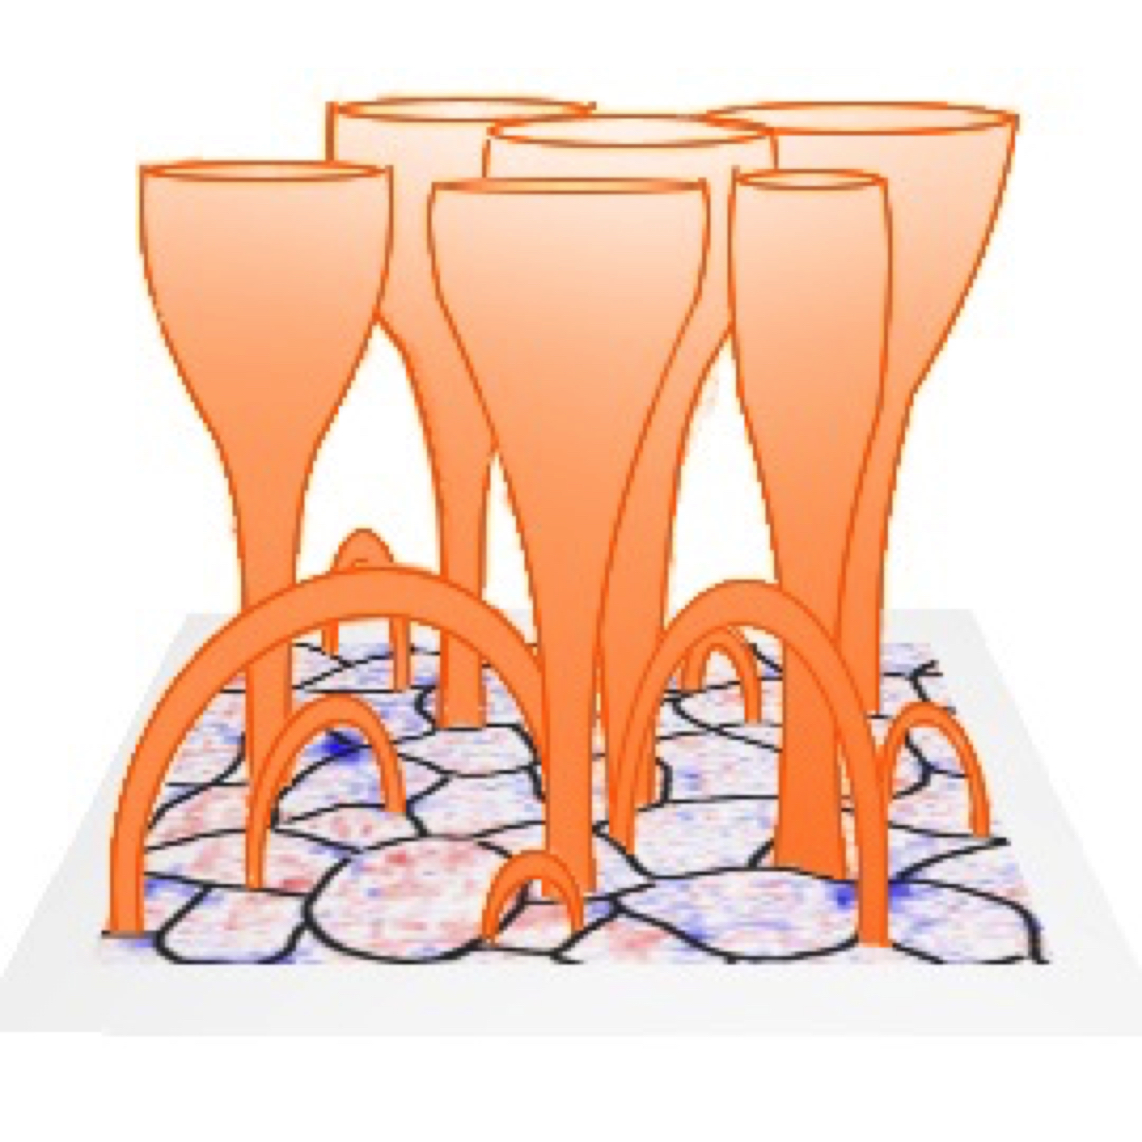
\includegraphics[scale=1.0]{solar-network-v1.jpg}
\caption{The schematic solar magnetic network.}
%\caption{Initial Magnetic Field Configuration, radial field distribution, uniform in the vertical direction with a maximum value of 100G }
\end{figure}

Active regions producing flares may have fields which easily exceed the normal range of 100-500 G. As well as these massive concentrations, solar magnetograms reveal many north poles in the quiet photosphere, this is known as the magnetic carpet. These structures can be observed in figure 1. Along with the coronal funnels arising from grain boundaries, the picture shows a range of network loops with temperatures which can be in the range $10^{5}$K to $10^{6}$K. The dynamical phenomena of concern in this paper result in waves and oscillations in the solar atmosphere. The upward propagation of waves through the solar atmosphere can result in coronal heating, frequency shifts and other wave phenomena. A range of wave transformations may occur including reflection and refraction by atmospheric structures. 


Our initial computational studies were applicable to quiet sun regions regions with magnetic fluxes in the range 5-10G this includes the non magnetic solar chromosphere and the quiet inter-network regions between the magnetic flux concentrations. Given the variety of solar atmosphere regions for example the network, inter network, plage and faculae regions it is recognised that the modes of oscillation with periods of 3 and 5 minutes exhibit varying behaviour. In particular is the variation observed for different magnetic structures and reflecting layers such as the transition layer which influences propagation in the upward and downward direction.


%%\begin{figure}[h]\label{VAL3C_rho_temp_fig1L}
%%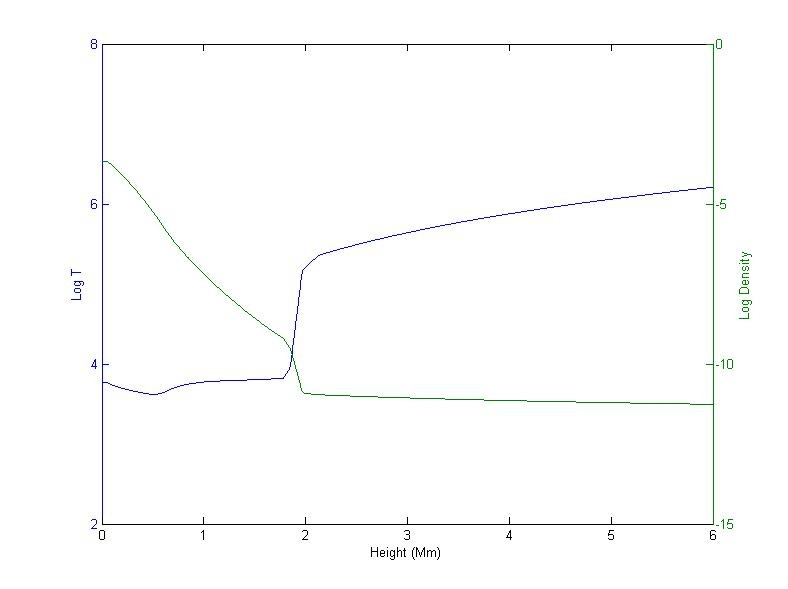
\includegraphics[scale=1.5]{VAL3C_rho_temp_fig1L.jpg}
%%\caption{Temperature and Density profile used for the simulations and based on the VALIIIc model.}
%%\caption{Initial Magnetic Field Configuration, radial field distribution, uniform in the vertical direction with a maximum value of 100G }
%%\end{figure}

%%\begin{figure}[h]\label{soundspeedVAL3C_profile_fig1R}
%%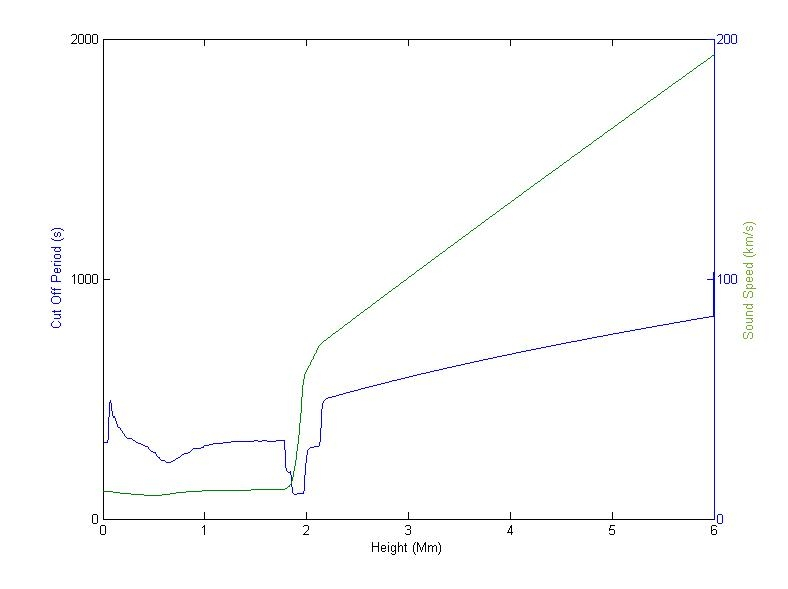
\includegraphics[scale=1.5]{soundspeedVAL3C_profile_fig1R.jpg}
%%\caption{Soundspeed and Frequency cutoff for a solar model atmosphere based on the VALIIIc model.}
%%\caption{Initial Magnetic Field Configuration, radial field distribution, uniform in the vertical direction with a maximum value of 100G }
%%\end{figure}








The power spectra presented in the first figure of \citet{Griffiths2018b} exhibit a variation of propagation characteristics at different levels within the solar atmosphere and within different regions such as coronal holes, the quiet sun and active regions. In general the power spectra indicate a preponderance of long period 5 minute waves with frequencies in the range 1.5-5mHz. Also observed are the distinctive peaks for the short period 3 minute waves (with frequencies in the range 5-8mHz). The power spectra exhibit peaks in much longer period ranges for example 12 minute waves  (frequencies in the range 1.1-1.5mHz)  and 16 minute waves (frequencies 1-1.1mHz). For the quiet sun regions the 5 minute modes are stronger at photospheric levels and diminished higher up in the corona, but note a small peak for the data from the AIA 211 corresponding to 2.0MK. 

%\begin{figure}[h]\label{powerspectra}
%\includegraphics[scale=0.5]{powerspectra.jpg}
%\caption{Power spectra}
%%\caption{Initial Magnetic Field Configuration, radial field distribution, uniform in the vertical direction with a maximum value of 100G }
%\end{figure}

The review of \citet{Khomenko2013} summarises this multifaceted picture. In the close proximity of the magnetic network elements, the longer 5 minute modes propagate efficiently to the chromosphere. The 3 minute modes propagate from the photoshere to the chromosphere in the network cell interiors for restricted regions of the network and internetwork. Although these long-period halos are present in the chromosphere they are most prominent in the photosphere. With their more complex magnetic structures, a more complex pattern is exhibited in plage and faculae regions. Observations show that the 3 minute modes exhibit enhancement in both photosphere and chromosphere whereas the power of the 5 minute modes increase significantly in the chromosphere. These power enhancements are known as “halos” and have been widely reported \citet{Kontogiannis2010}. 





\section{Motivation} \label{sec:motivation}

Given the complexity of the dynamics and the diversity of structures in the solar atmosphere, it is understood that a truly realistic model is challenging and requires a hybrid multi-disciplined approach. In order to develop a model providing a representation of the solar atmosphere it is necessary to establish that the modelling tools give a consistent behaviour in idealised test cases and that there is a consistency between the computational and theoretical models. Many computational MHD simulations of the sun have been undertaken, some of the approaches have resulted in an encouraging degree of realism  \citet{Vogler2005}, \citet{Gudiksen2011}. Computational MHD simulations of the propagation of waves in 3D solar atmospheres were undertaken by \citet{Fedun2009a}. Initially they considered hydrodynamical models, in later simulations \citet{Fedun2009b} \citet{Vigeesh2012} reported results for magnetized solar atmospheres featuring an idealized flux tube. These models with point drivers demonstrated the leakage of magneto-acoustic energy into the solar atmosphere. The work of \citet{Khomenko2013} and  \citet{Santamaria2015} reviewed and presented 2D computational MHD modelling of wave propagation in magnetic features such as sunspots and arcades. 

 
The models reveal that vertical magnetic fields enable energy to reach the corona. Our initial models of a realistically stratified model of the solar atmosphere \citet{Griffiths2018b} were hydrodynamic simulations. In these simulations atmospheric perturbations caused by photospheric global oscillations are represented using drivers located in the photosphere so as to mimic the influence of the solar p-modes. The results of the hydrodynamic modelling exhibited agreement  with the energy flux predictions from a 2 layer Klein-Gordon model. This agreement supported the interpretation of the interaction between the solar atmosphere and the global oscillations. Also revealed by the simulations  was a consistency between power flux measurements from SDO and frequency dependent energy flux measurements from the numerical simulations. This observed propagation of energy into the mid to upper atmospheric regions of the quiet sun occurred for a range of frequencies. Such observations may explain observed intensity oscillations for periods greater than the well known 5-minute and 3-minute oscillations. It was also found that energy flux propagation into the lower solar corona is strongly dependent on the particular wave modes. 


In this paper we present results for 3D numerical MHD simulations with an extended driver representing photospheric p-mode oscillations in a magnetic solar atmosphere, the objective is to gain understanding of the propagation characteristics of the p-mode oscillations. 




\section{Numerical Computation Methods}


The simulations described in in this paper were undertaken using the SMAUG code, a GPU implementation of the Sheffield Advanced Code (SAC) \citet{Shelyag2008}. The Sheffield MHD Accelerated Using GPUs (SMAUG) \citet{Griffiths2015} and SAC  are derived from the versatile advection code (VAC) developed by \citet{Toth1996}. SAC and SMAUG are numerical MHD solvers which can be used to model the time-dependent evolution of photospheric oscillations in the solar atmosphere. The SMAUG code can simulate linear and non-linear wave propagation in strongly magnetised plasma with structuring and stratification.

We use the same general system of ideal MHD equations applicable to an ideal compressible plasma and used for our initial hydrodynamic simulations, \citet{Griffiths2018b}.
\begin{eqnarray}
&& {{\partial \rho}\over{\partial t}}+\nabla\cdot\left( \rho{\mathbf v}\right)=0, \label{e1} \\
&& {{\partial ( \rho {\bf v})}\over{\partial t}}+\nabla\cdot\left( {\bf v}\rho {\bf v}-{\bf B B}\right)+\nabla p_t=\rho{\bf g}, \label{e2}\\
&& \frac{\partial e}{\partial t}+\nabla\cdot\left({\bf v}e-{\bf B B}\cdot{\bf v}+{\bf v}p_{t}\right)+\nabla p_t=\rho{\bf g}\cdot{\bf v}, \label{e3} \\
&& {{\partial{\bf B}}\over{\partial t}} +\nabla \cdot\left(  {\bf vB}-{\bf Bv}\right)=0. \label{e4}
\end{eqnarray}


The total pressure $p_{t}$ is given by
\begin{equation}
p_{t}=p_{k}+{{\bf B}^{2}\over{2}}, \label{e5}
\end{equation}
and the kinetic pressure, $p_k$, is written as
\begin{equation}
p_{k}=\left(\gamma -1\right)\left(e-\frac{\rho {\mathbf v}^{2}}{2}-\frac{{\mathbf B}^{2}}{2}\right). \label{e6}
\end{equation}

In the system of equations above,  $\mathbf B$ is the magnetic field, $\mathbf v$ is the velocity, $\rho$ is the mass density, $\mathbf g$ is the gravitational acceleration vector  and  $\it{e}$ is the energy density. The SMAUG code used for the simulations reported here employs perturbed versions of the general set of MHD equations given above. For the perturbed versions the density,  energy density and magnetic field are expressed in terms of perturbed and background quantities as follows
\begin{eqnarray}
&& \rho = \tilde{\rho}+\rho_b, \nonumber \\
&& e = \tilde{e}+e_b,  \nonumber \\
&& {\mathbf B} = \tilde{\mathbf B}+{\mathbf B}_b.  \nonumber 
\end{eqnarray}
Assuming a magneto-hydrostatic equilibrium of the background plasma, the background quantities which do not change in time have a subscript $\it{b}$. The time varying perturbed quantities do not have a subscript. The fully non-linear MHD numerical finite element solver employs hyper-diffusion and hyper-resistivity to achieve numerical stability of the computed solution of the MHD equations \citet{Caunt2001}. A more detailed description of the full set of MHD equations, including the hyper-diffusion source terms are given in \citet{Griffiths2015} and \citet{Shelyag2008}.

\begin{figure}[h]\label{inimagfieldplot}
\centering
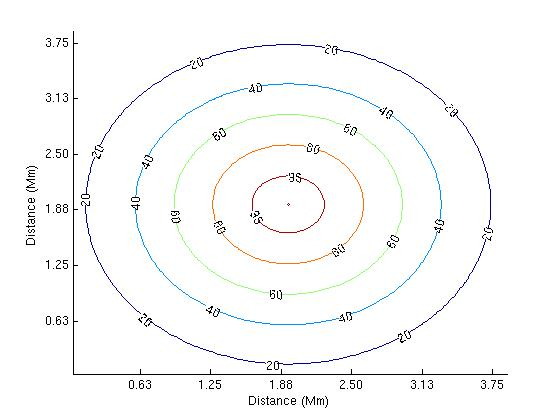
\includegraphics[scale=0.2]{bfield100G.jpg}
\caption{Initial Magnetic Field Configuration, radial field distribution, uniform in the vertical direction with a maximum value of 100G }
\end{figure}

\break

\section{Computational Model}
The hydrodynamical studies reported in  \citet{Griffiths2018b} employed simulation drivers with physical characteristics representing p-mode oscillations with varying modes and periods. The MHD simulations reported here use the same driver and model of the solar atmosphere as used in our initial hydrodynamical study. The model is modified by the inclusion of a uniform, vertical and cylindrically symmetric magnetic field. 

 The dimensions of the simulation box are $L_{ x}= 4$ Mm,  $L_{y} =4$ Mm and with a height of $L_{z} =6$ Mm in the gravitationally stratified $z$-direction. The computational box is an array of elements $128 \times128 \times128 $. The upper boundary of the model is in the solar corona whilst the lower boundary is coincident with the photosphere. The perturbed MHD code used here is suited to studying the propagation of wave energy from the photosphere, across the transition layer and leaking into the solar corona. The time scales relevant to our study are determined by the 5-minute $p$-mode oscillations the model employs open boundary conditions thereby allowing us to model the wave propagation. To generate these oscillations we use vertical velocity drivers which are extended across the base of the model. The following sections describe the model solar atmosphere and the driver.

Data obtained from solar observations was used to construct a semi-empirical model solar atmosphere, the resulting model is a representation of the quiet sun. Employing the fundamental assumption of hydrostatic equilibrium, the VALIIIc model \citet{Vernazza1981} was used to construct a model of the chromosphere in equilibrium. For atmospheric heights greater than 2.5 Mm the results from a model of solar coronal heating were used \citet{McWhirter1975}. The atmospheric profiles for temperature, density, sound speed and frequency cut-off for this model are shown in figure \ref{soundspeedVAL3C_profile_fig1R}. A further possiblity for a model solar atmosphere is the use of parametric models, the smoothed step function used by \citet{Murawski2010} is an example. Discussion of the validity of model solar atmospheres and realistic models of the chromosphere,  indicate the need for observationally derived semi-empirical models, see \citet{Carlsson1995}, \citet{Kalkofen2012}. It has been suggested that local dynamo action and joule heating in the dynamical solar chromosphere make the construction of models particularly challenging \citet{Leenaarts2011}.

For the simulations described here we use a simplistic model which is uniform in the vertical (z) direction. The cylindrically symmetric field was constructed using  the parametrisation in equation \ref{e7}, the effective cylinder radius was fixed at $R=0.14$Mm. Simulations were run for different values of $B_{max}$.

\begin{equation}
B_{z}=B_{max} e^{-\frac{x^2+y^2}{R^2}} , \label{e7}
\end{equation}

Since the field is uniform in the vertical direction the model atmosphere is in magnetohydrostatic equilibrium. Details of the construction procedure for the model atmosphere, the resulting density profiles and temperature profiles are provided in \citet{Griffiths2018b}. 
 
\begin{figure}[h]\label{soundspeedVAL3C_profile_fig1R}
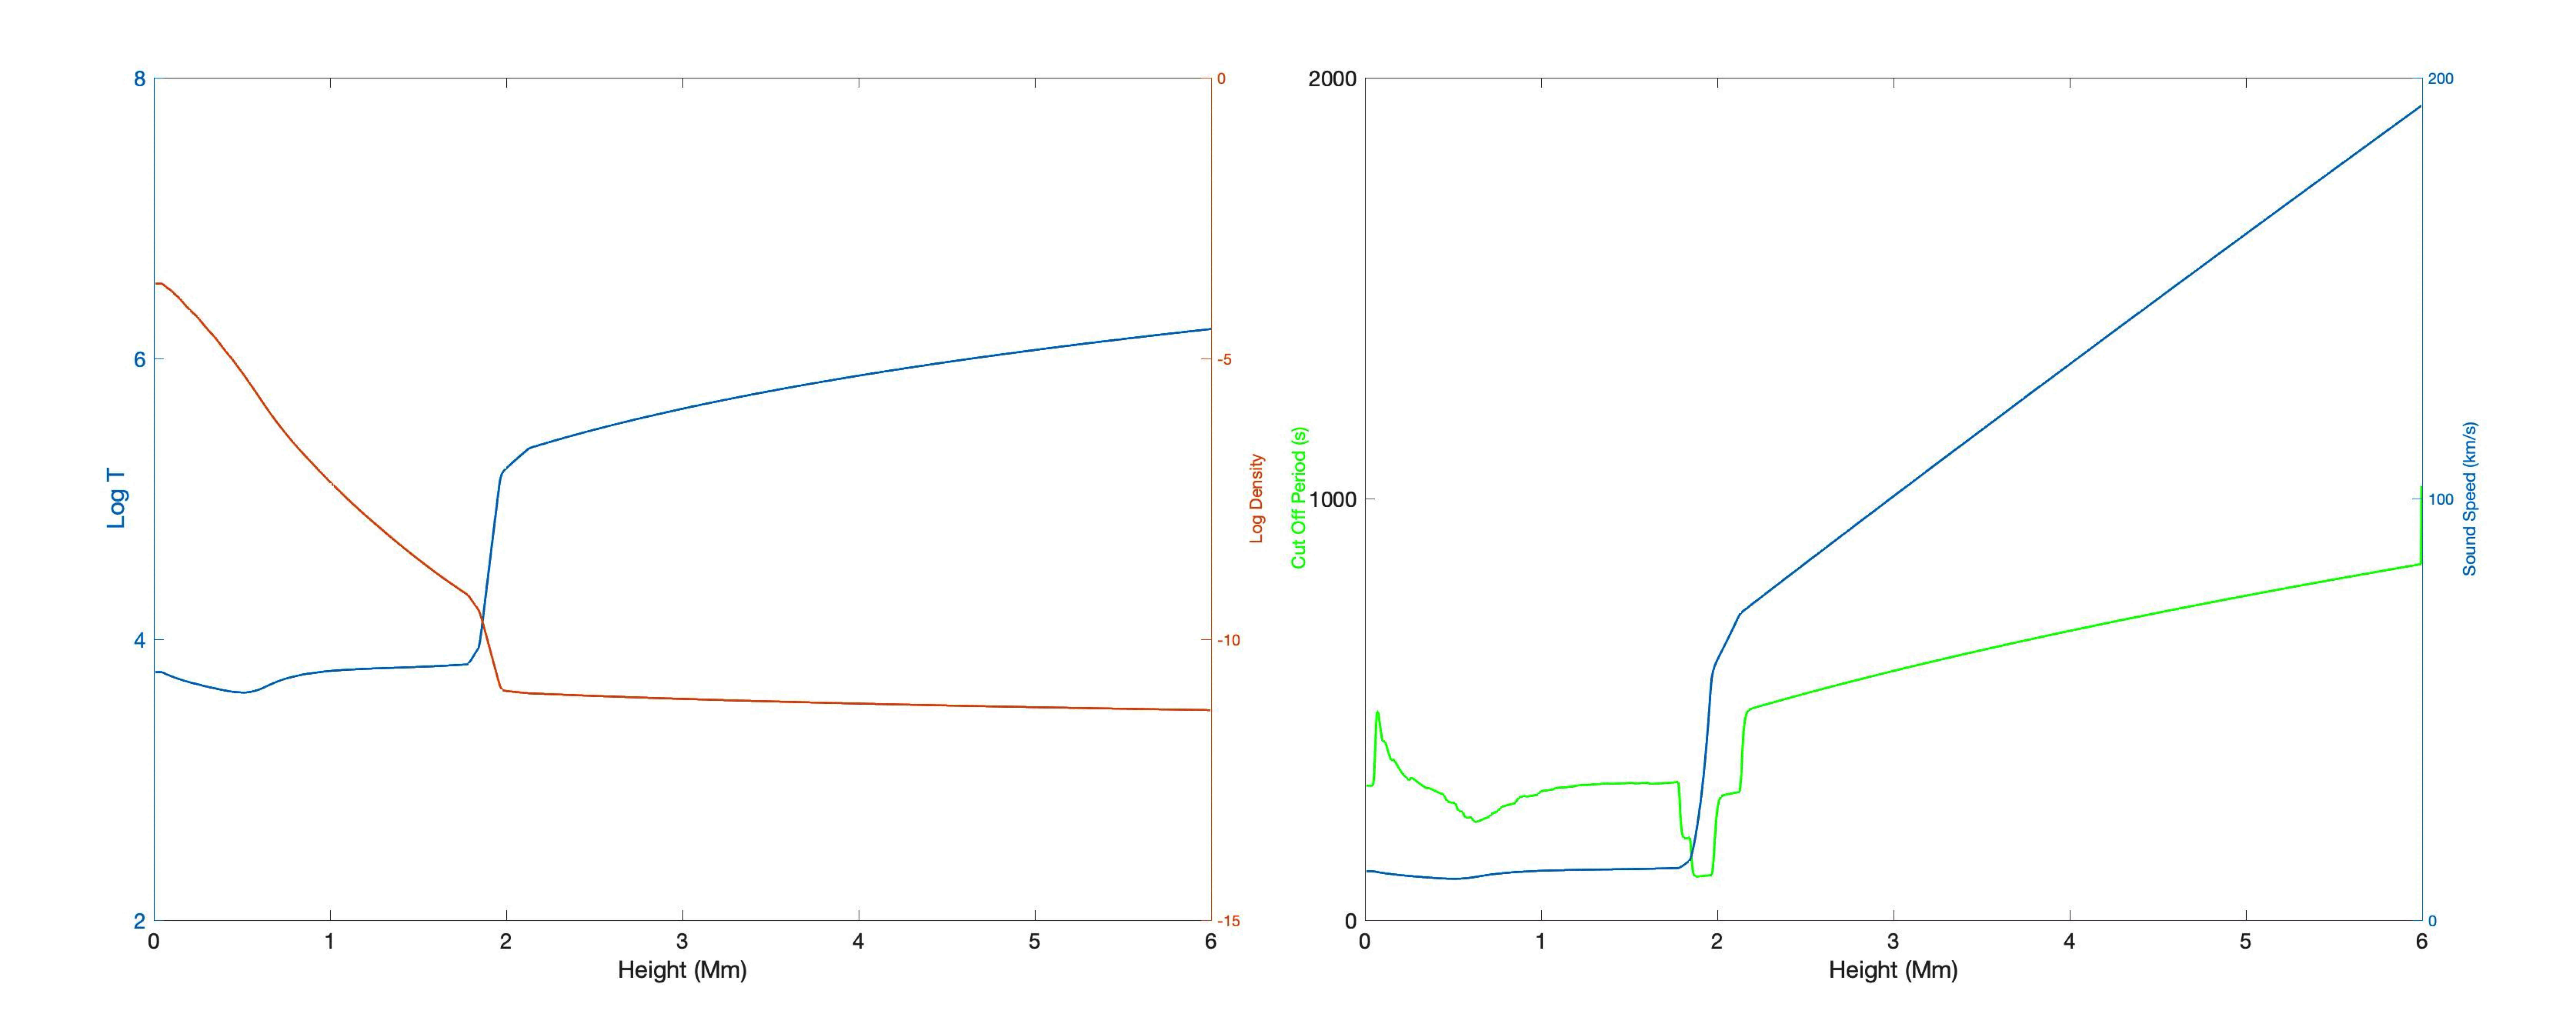
\includegraphics[scale=0.15]{solatmosprofiles.jpg}
\caption{The left hand panel shows the temperature and density profile used for the simulations and based on the VALIIIc model. The right hand panel shows the computed soundspeed and frequency cutoff for a solar model atmosphere based on the VALIIIc model.}
%%\caption{Initial Magnetic Field Configuration, radial field distribution, uniform in the vertical direction with a maximum value of 100G }
\end{figure}

\section{Numerical Drivers for $p$-mode Oscillations}

The work reported here is an extension of the earlier work of \citet{Malins2007}, their study represented photospheric buffeting motion using different point drivers. These studies demonstrated surface waves, structures in the transition zone and identified the effect of cut-offs induced by the stratified  solar atmosphere. The overview in Section 2 identified physical phenomena delivering energy into the solar atmosphere and resulting in oscillatory behaviour. 

The simulations presented in this paper, employ an extended driver resulting in the perturbation of the entire lower boundary of the model.  Photospheric $p$-mode oscillations for the real sun have a horizontal wavelength and coherence. The vertical velocity driver used here is an acoustic $p$-mode driver located at the photosphere and exciting waves which propagate 
into our realistic 3D model of the solar atmosphere. An extended driver with a sinusoidal dependence and a wavelength of 8 Mm applied along the middle of the base of a computational domain of dimension 4 Mm represents  a {\it fundamental mode}. Drivers may be constructed as an ensemble of these solar global eigenmodes. The driver is represented by the expression shown in equation (\ref{e8}) 


%%\begin{tabular}{ccc}
\begin{equation}
 V_{z}  =  A_{nm} \sin\left(\frac{2\pi t}{T_s} \right)\sin\left(  \frac{(n+1)\pi x}{L_x} \right)  
 \sin\left(\frac{(m+1)\pi y}{L_y} \right) \exp\left( -\frac{(z-z_0)^2}{\Delta z^2} \right),
\label{e8}
\end{equation}
%%\end{tabular}

For the  simulations here, a p-mode driver corresponding to the 5 minute mode, was used with period 300s and mode (2,2). Earlier studies demonstrated the effectiveness of this mode with energy propagation. Simulations were run for different values of the magnitude of the magnetic field. The mode numbers identified here are the n and m values in the expression for the driver shown in equation (\ref{e8}).


\begin{figure*}\label{vzplot_bv100g_76_150_225}
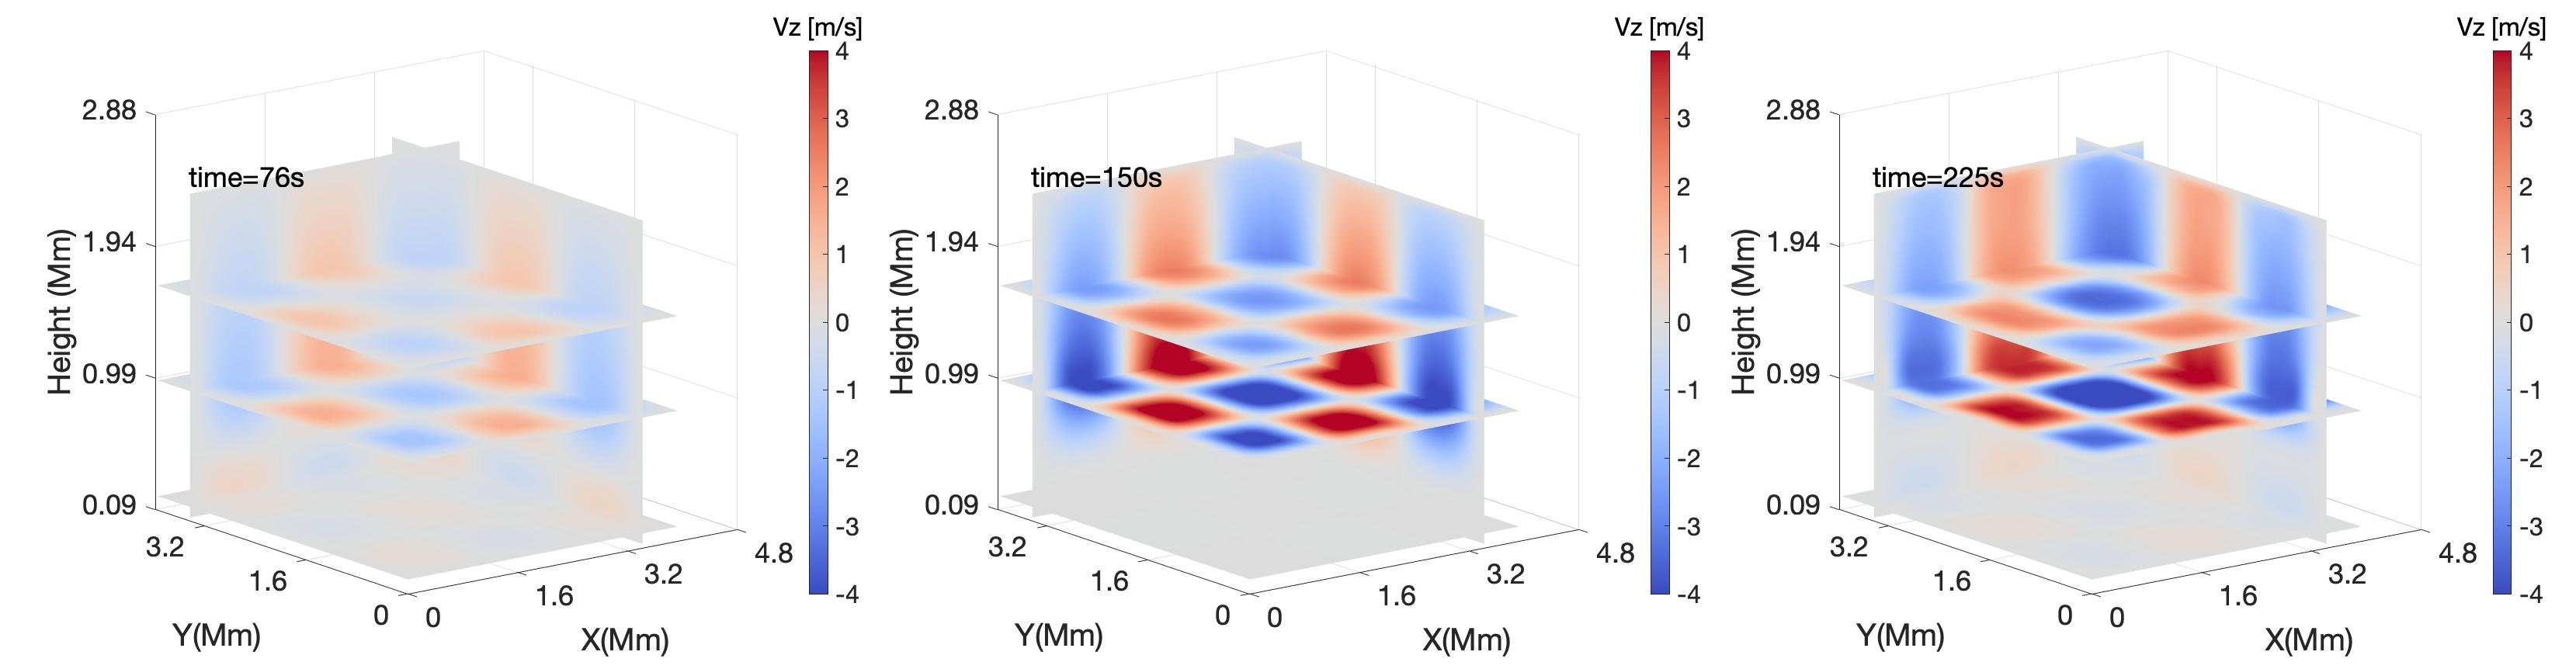
\includegraphics[scale=0.146]{vz_bv100g_76_150_225.jpg}
\caption{Vertical Component of the Velocity for Different Sections of the Simulation for 76s, 150s and 225s for a vertical field with maximum field of 100G.}
%\caption{Initial Magnetic Field Configuration, radial field distribution, uniform in the vertical direction with a maximum value of 100G }
\end{figure*}



\begin{figure*}\label{vzplot_bv0g_76_150_225}
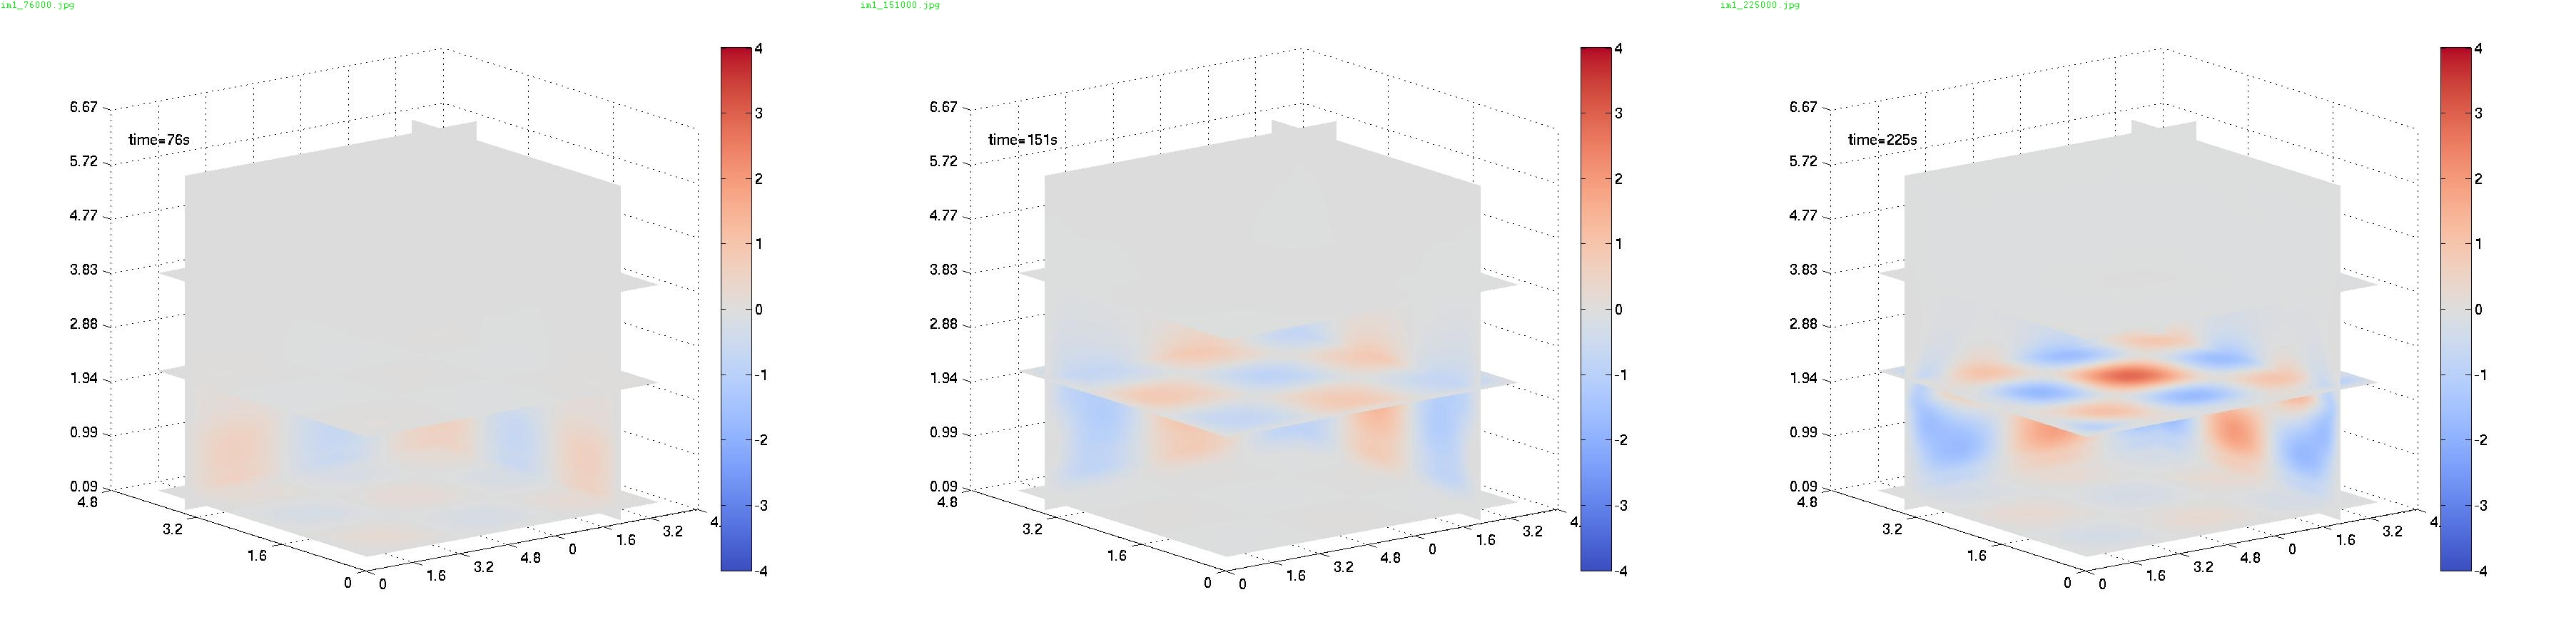
\includegraphics[scale=0.146]{vz_bv0g_76_150_225.jpg}
\caption{Vertical Component of the Velocity for Different Sections of the Simulation for 76s, 150s and 225s for a magnetic field of 0G.}
%\caption{Initial Magnetic Field Configuration, radial field distribution, uniform in the vertical direction with a maximum value of 100G }
\end{figure*}



%\begin{figure*}\label{vzplot_bv100g_0g_76_150_225}
%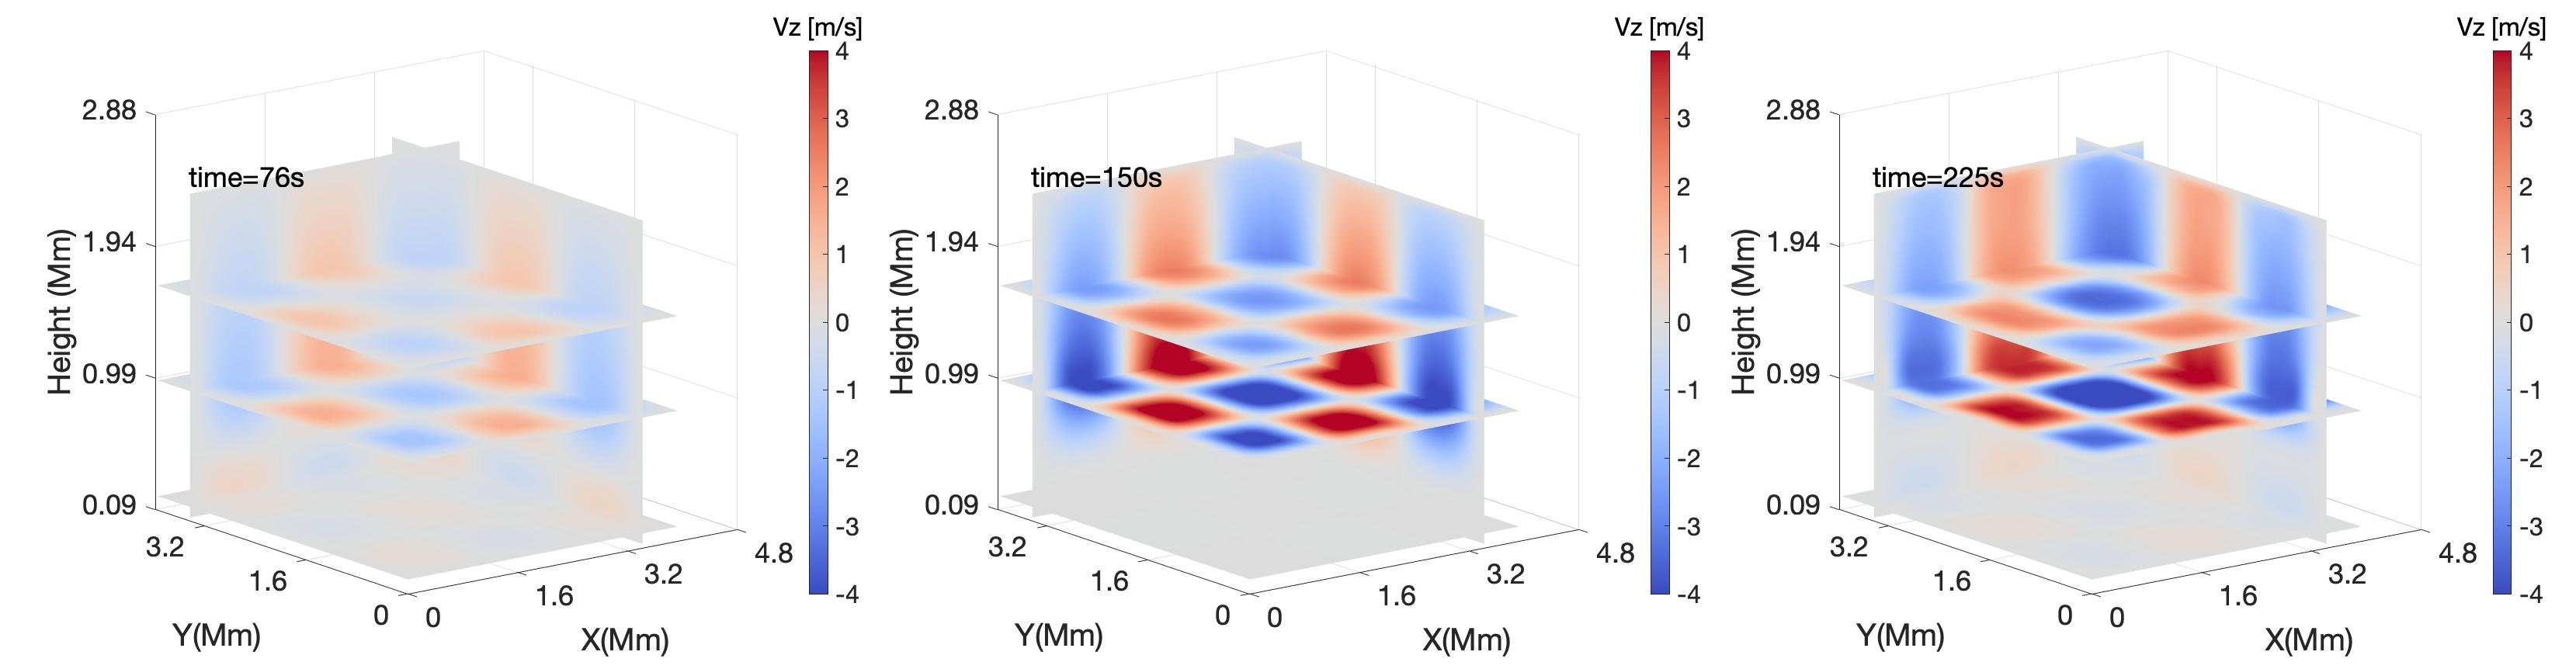
\includegraphics[scale=0.146]{vzplot_bv100g_76_150_225.jpg}
%\caption{Vertical Component of the Velocity for Different Sections of the Simulation for 76s, 150s and 225s for a magnetic field of 100G.}
%\caption{Initial Magnetic Field Configuration, radial field distribution, uniform in the vertical direction with a maximum value of 100G }
%\end{figure*}


For the driver equation given in \ref{e8}, $T_{s}$ is the period, $A_{nm}$ is the amplitude, the indices $n$ and $m$ define the mode, the lengths of the base of the simulation box in the $x$ and $y$ directions are $L_{x}$ and $L_{y}$ are  respectively. The driver width, $\Delta z$ is set to $4$km, the parameter $z_{0}$ was set so that the vertical location of the driver is in the photosphere, coincident with the location of the temperature minimum and 0.5 Mm above the lower boundary of the model. The simulations presented use the parameter $A_{nm}$=500\, ms$^{-1}$ with the mode indices set to $n,m=2$. 




%\ref{vzplot_bv0g_76_150_225} , \ref{vzplot_bv50g_76_150_225} , \ref{vzplot_bv75g_76_150_225} and 

\section{Magnetoacoustic Waves in Uniform Vertical Magnetic Field Configurations}
Magnetohydrodynamic simulations have been performed with p-mode oscillations of the photospheric layer and for magnetic field strengths of 0G, 50G, 75G and 100G. The plasma $\beta$ for the model decreases rapidly from a value of 50 at 0.7Mm above the lower boundary of the simulation domain, $\beta$ decreases to 1 at a height of 1.39Mm.  It is anticipated that for the region with $\beta \approx 1$, mode conversion occurs with full or partial conversion to magnetohydrodynamic modes. 

 %% Figure 3  \ref{vzplot_bv100g_76_150_225}
 Figure \ref{vzplot_bv100g_76_150_225} shows the vertical component of the velocity at various times for different sections through the simulation box. Each plot in  figure \ref{vzplot_bv100g_76_150_225} corresponds to a vertical field configuration with a maximum field strength ( $ B_{max} $ ) of 100G. Comparison with the 0G case in figure \ref{vzplot_bv0g_76_150_225}, illustrates a clear difference between the purely hydrodynamic and the MHD case. The figures for the MHD case exhibit evidence of a fast moving magneto-acoustic wave mode. These figures compare the wave modes at a quarter, half and three-quarters of a cycle. The propagation speed is consistent with that of a fast magneto-acoustic mode. Our results indicated that even a small magnetic field appears to enhance the motion of plasma in the corona and  there is an apparent difference in phase between the magnetic field cases. As well as an increase in the velocity amplitude with increasing magnetic field there is a small shift in the frequency of the oscillation. For magnetic fields with strengths between $1$kG and$50$G, the theoretical prediction of \citet{Hindman1996} resulted in frequency shifts in the microhertz and nanohertz range,  although this was a helioseismology prediction it provides insight into the mechanism of frequency shifts of waves in atmospheric magnetic structures. 

A set of videos of all the simulations that were performed can be obtained from the online research data archive hosted by The University of Sheffield \citet{Griffiths2018a}. The videos display the evolution of the $z$-component of the plasma velocity along different layers of our model solar atmosphere. Each video shows the value of the vertical component of the plasma velocity ($z$-component in m/s) along different slices through the simulation box. Each video is labelled using the magnetic field strength in Gauss.






%Figure \ref{dt_vvert_5b2_2_2Mm_1Mm_0p5MM_0G_25G_50G_100G_line} 
%Figure \ref{dt_vvert_100G_300s_180s}

%Figure \ref{dt-5b2_2_100G-midchrom} shows a plot of the z component of the velocity at different times for a location at the centre of the box. Different curves are plotted for different heights. The red, green and blue curves correspond to a height  of 0.5Mm, 1Mm and 2Mm respectively. Although the periods are the same as that of the driver there are different shifts for different heights the shift corresponds to the propagation time for that height. The velocities for the magnetic field cases are larger than for the field free case.

%Time distance plots for the model with the 100G field are shown in figure  \ref{dt_vvert_100G_300s_180s_1p4Mm} these plots show %the case of the driver period of 300s and 180s. 

% figure \ref{dt_vvert_100G_300s_180s}
A distance-time plot for the 300s period driver, with the 100G field is shown in figure 4. The wavespeeds computed from this distance-time plot are shown in table \ref{Tablewavespeeds_300s}. The speeds for the 0G field are consistent with the speed of sound in the solar atmosphere, whilst the speeds for the non zero magnetic field are consistent with propagation speeds for magnetosonic modes. 
\begin{table}\label{wavespeeds}
\centering
\begin{tabular}{c c c c c}
\hline
Wave Speed (km/s)   &  0G  &  50G &  75G & 100G\\
\hline
2Mm & 12.6  &   96.5       &   47.7      &  25.2     \\
\hline
1Mm & 10.1  &    64.1      &   44.4     &   45.4      \\
\hline
0.5Mm & 8.7  &   45.4      &   37.8      &   32.3    \\
\hline

\end{tabular} 
\caption{The table shows wave speeds obtained from the distance-time plots for the 300s period driver with magnetic fields of 0G,50G, 75G and 100G.}
\label{Tablewavespeeds_300s}
\end{table}

\begin{table*}\label{energyflux}
\centering
\begin{tabular}{c c c c c}
\hline
Magnetic Field (G)   &  1Mm  &  2Mm &  4Mm & 5.5Mm \\
\hline
0G & 0.155  &    -1.771 x $10^{-5}$      &   1.227 x $10^{-6}$     &   8.194 x $10^{-7}$      \\
\hline
50G & 0.270  &   -0.399       &   0.040      &  0.021     \\
\hline
75G & -0.507  &    -0.126      &   0.015     &   0.007      \\
\hline
100G & -0.255  &   -0.226      &   0.019      &   0.006    \\
\hline

\end{tabular} 
\caption{The table shows the time averaged and integrated energy flux ratio obtained  for the 300s period driver with magnetic fields of 0G,50G, 75G and 100G.}
\label{energyfluxratio}
\end{table*}


 In the lower region of the model atmosphere the simulations exhibit evidence of slow magnetoacoustic wave propagation perpendicular to the field lines. Since the source terms perturb only the vertical component of the velocity and the model is cylindrically symmetric, pure Alfvenic modes are not expected. 


%PLOTCHANGE OF VELOCITY -Z WITH TIME AT DIFFERENT SECTIONS



%\begin{figure}[h]\label{vz_0G_50G_75G_100G_76}
%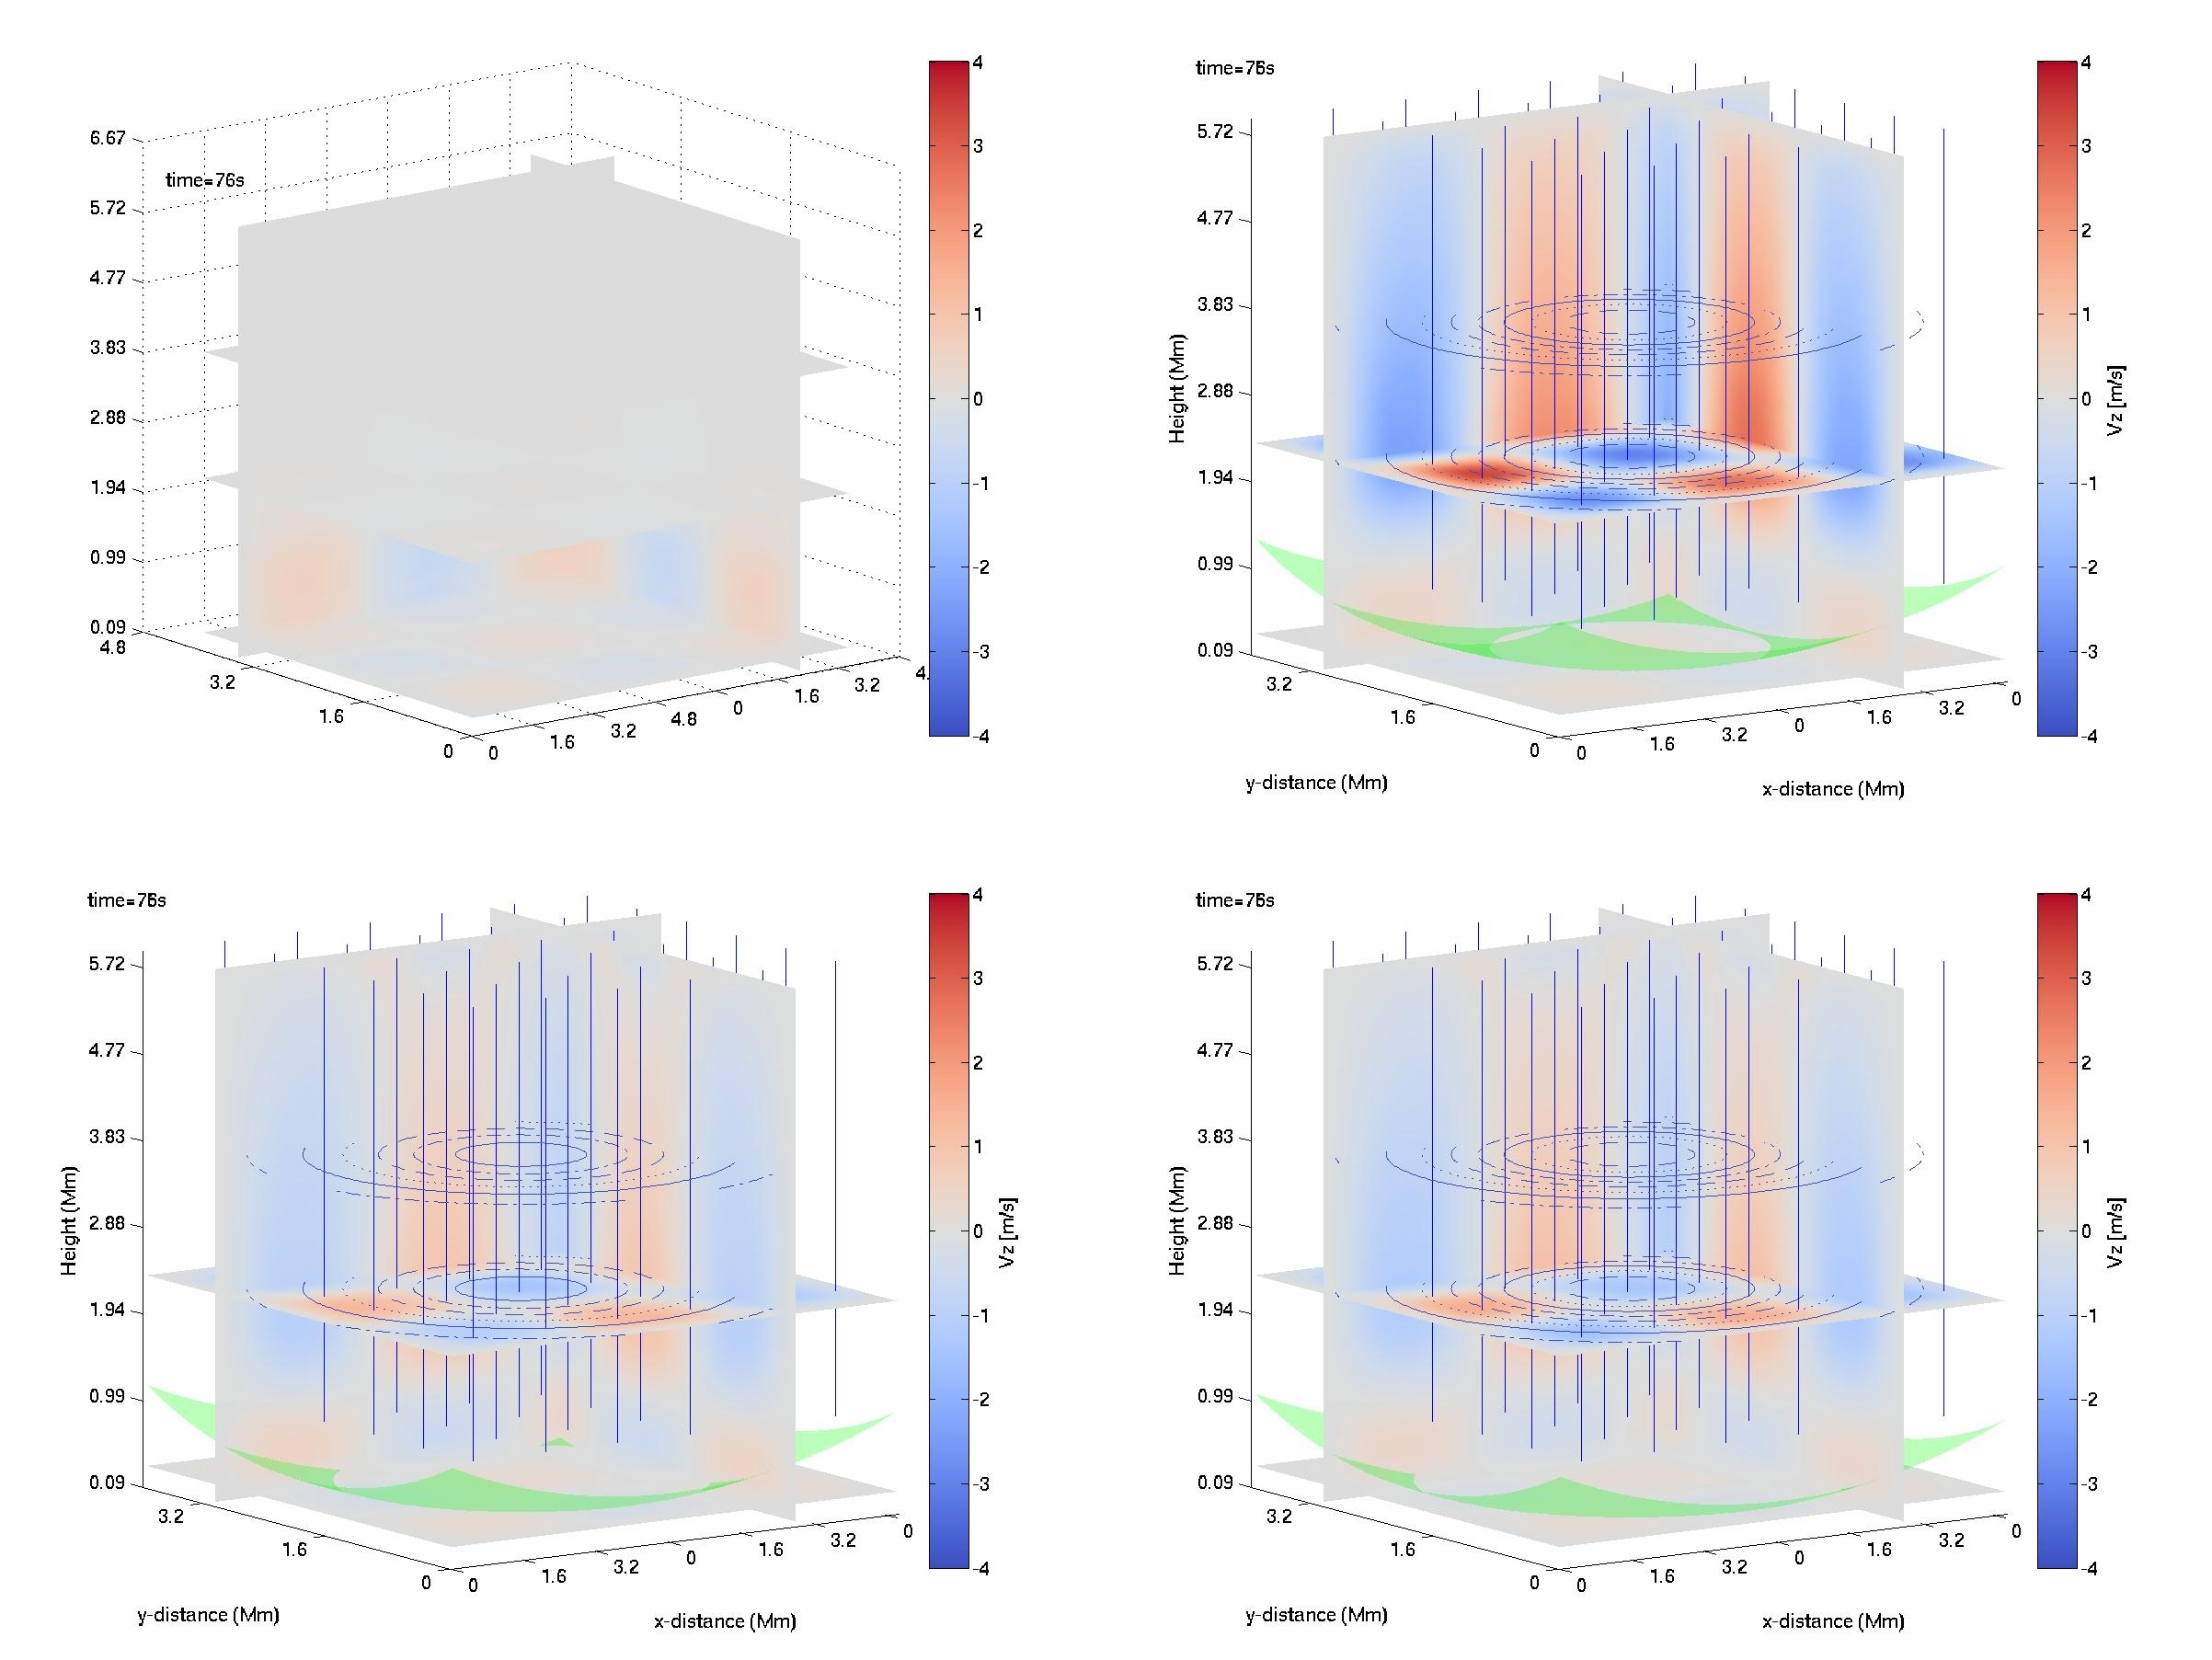
\includegraphics[scale=0.15]{vz_0G_50G_75G_100G_76.jpg}
%\caption{Vertical Component of the Velocity for Different Sections of the Simulation for 76s, comparing different strengths for the vertical field magnetic field of 0G, 50G, 75G and 100G}
%\caption{Initial Magnetic Field Configuration, radial field distribution, uniform in the vertical direction with a maximum value of 100G }
%\end{figure}

%\begin{figure}
%\centering
%\label{td_vert_bv100G_300_with_bandbeta}
%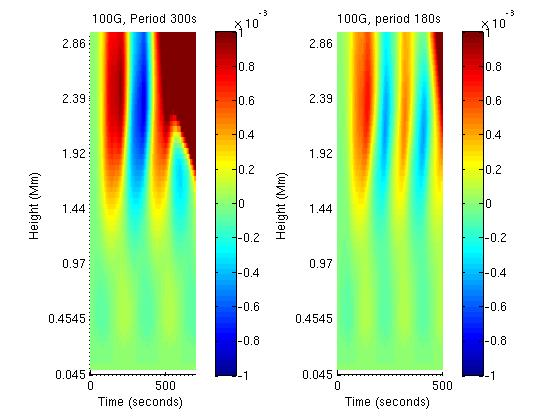
\includegraphics[scale=0.475]{dt_vvert_100G_300s_180s.jpg}
%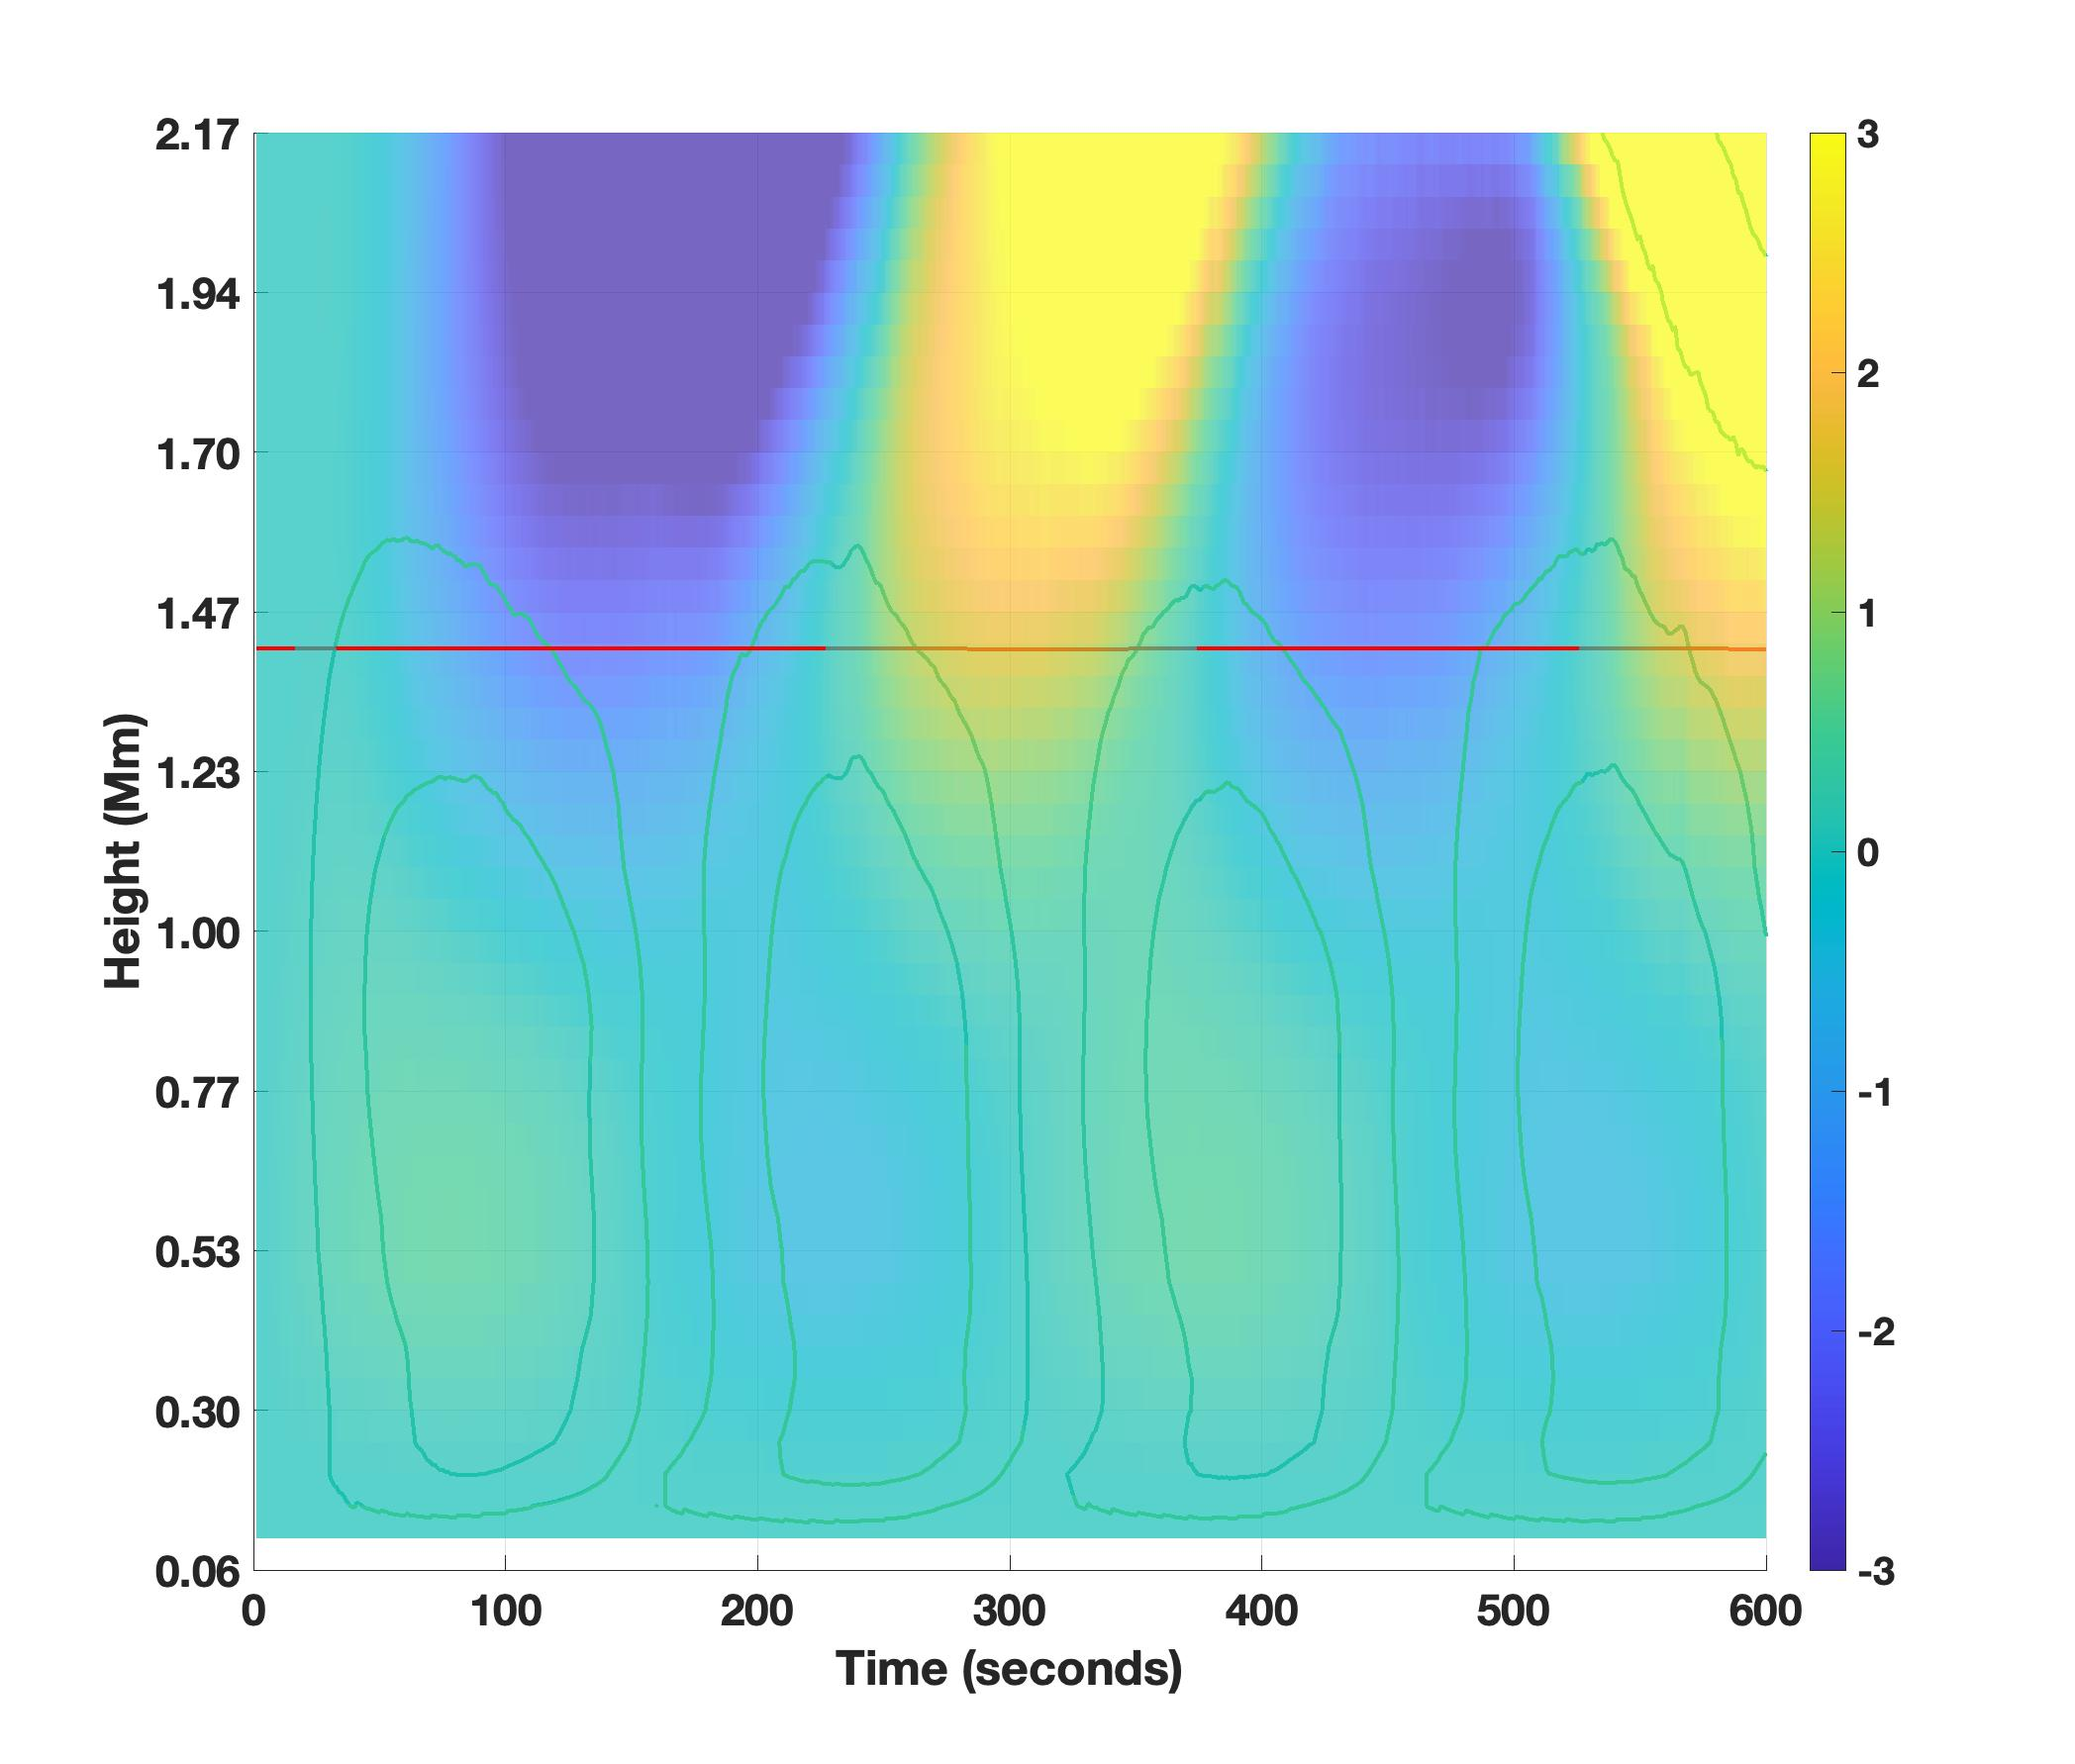
\includegraphics[scale=0.25]{td_vert_bv100G_300_with_bandbeta.jpg}
%\caption{Distance-time plot of the vertical component of the velocity in the mid chromosphere, contours show the reciprocal of the plasma beta also shown are contours for the perturbed magnetic field.}
%\caption{Energy Flux for the mid-section of the Simulation for 76s, 150s, 225s and 330s for a vertical field with maximum field of 50G }
%\end{figure}

\begin{figure}
\centering
\label{td_vert_bv0G_300}
%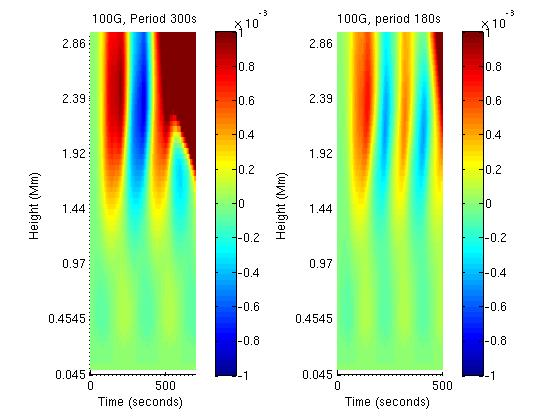
\includegraphics[scale=0.475]{dt_vvert_100G_300s_180s.jpg}
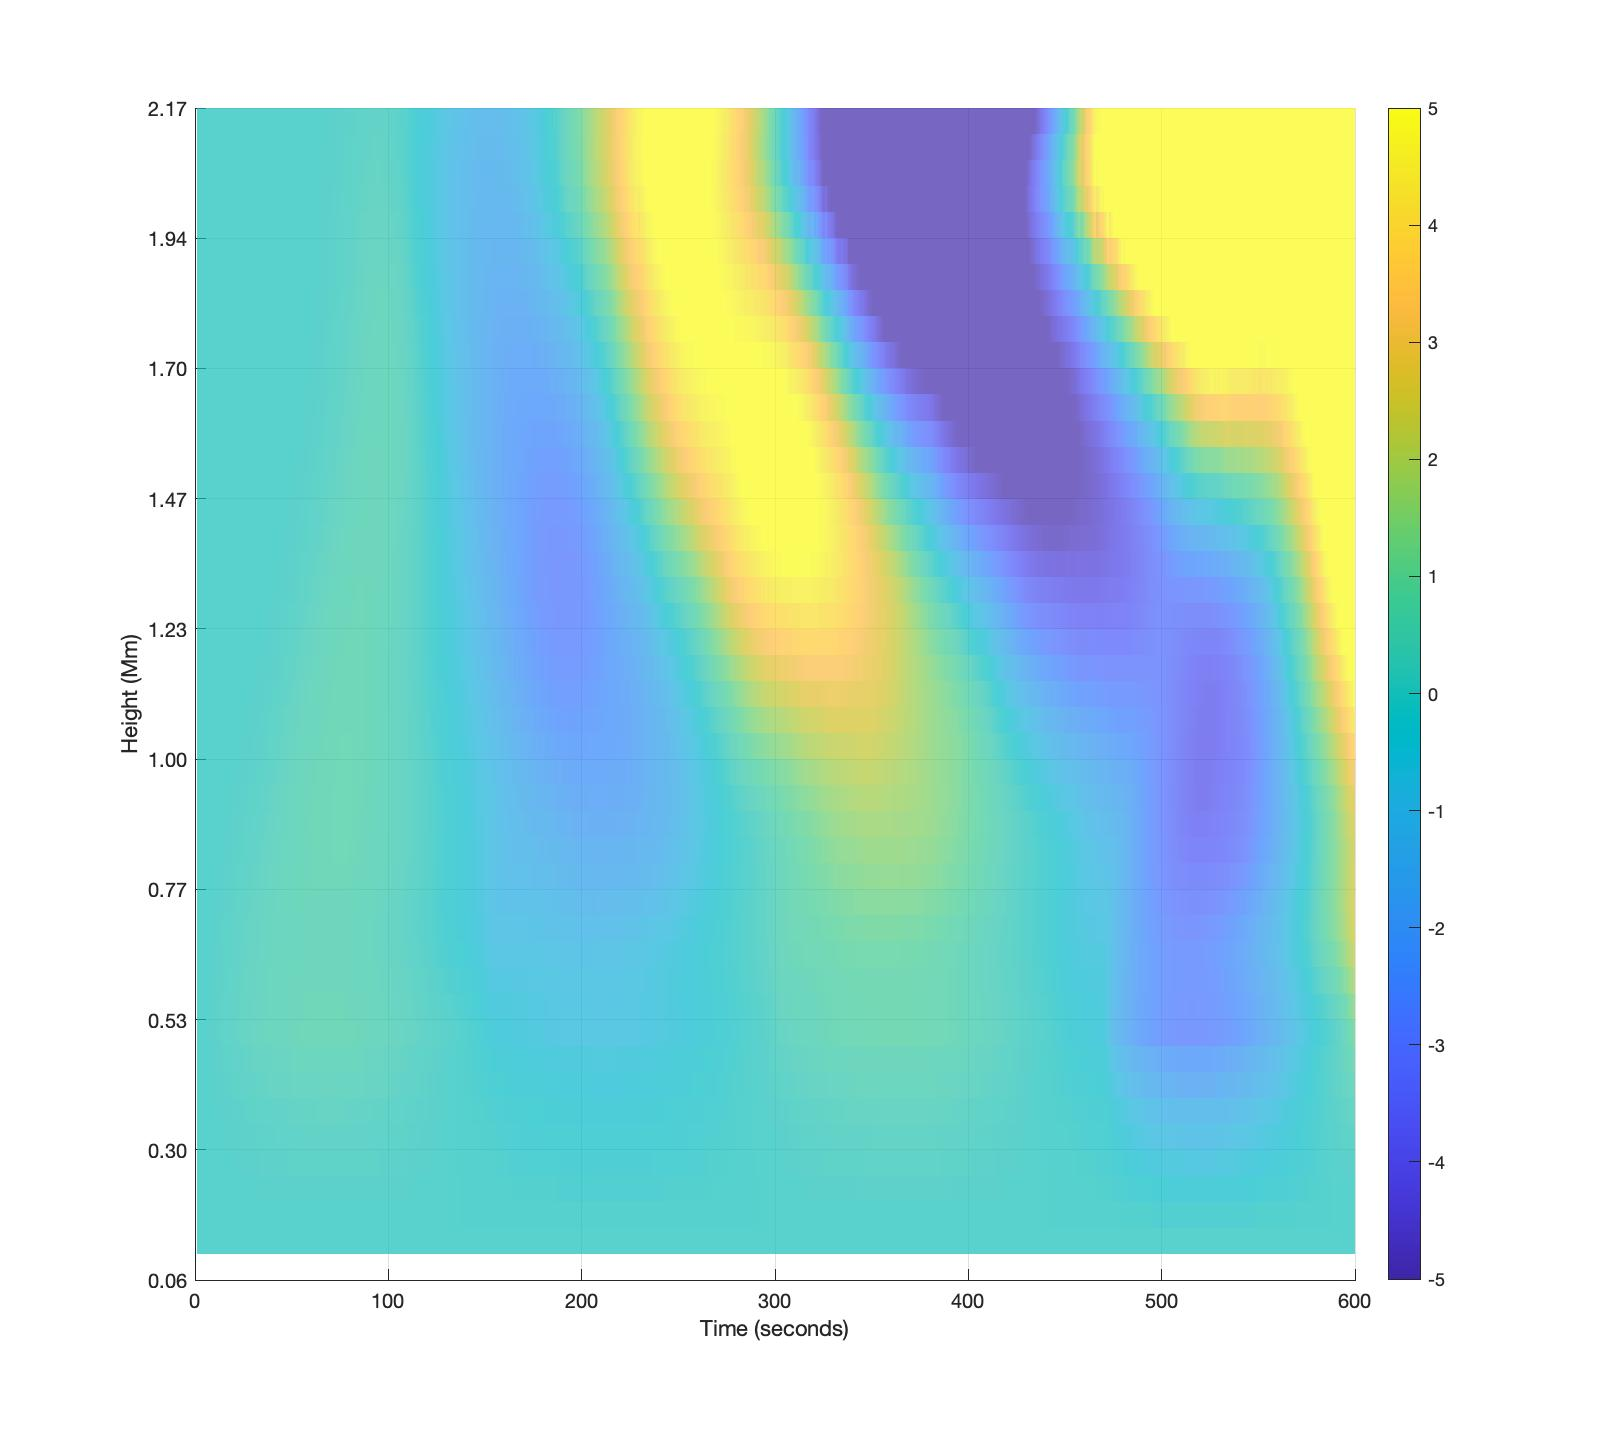
\includegraphics[scale=0.25]{td_vert_bv0G_300.jpg}
\caption{Distance-time plot of the vertical component of the velocity in the mid chromosphere, for the case with magnetic field of 0G}
%\caption{Energy Flux for the mid-section of the Simulation for 76s, 150s, 225s and 330s for a vertical field with maximum field of 50G }
\end{figure}


\begin{figure}
\centering
\label{td_vert_bv100G_300_with_bandbeta}
%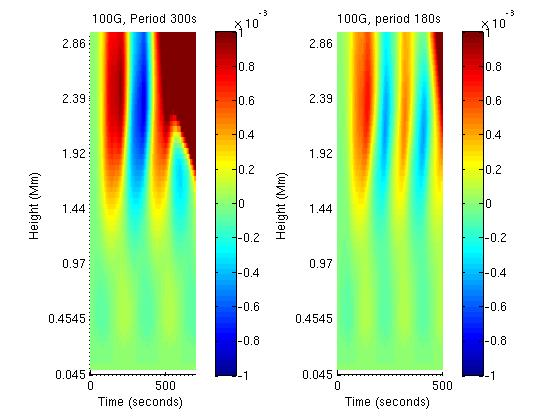
\includegraphics[scale=0.475]{dt_vvert_100G_300s_180s.jpg}
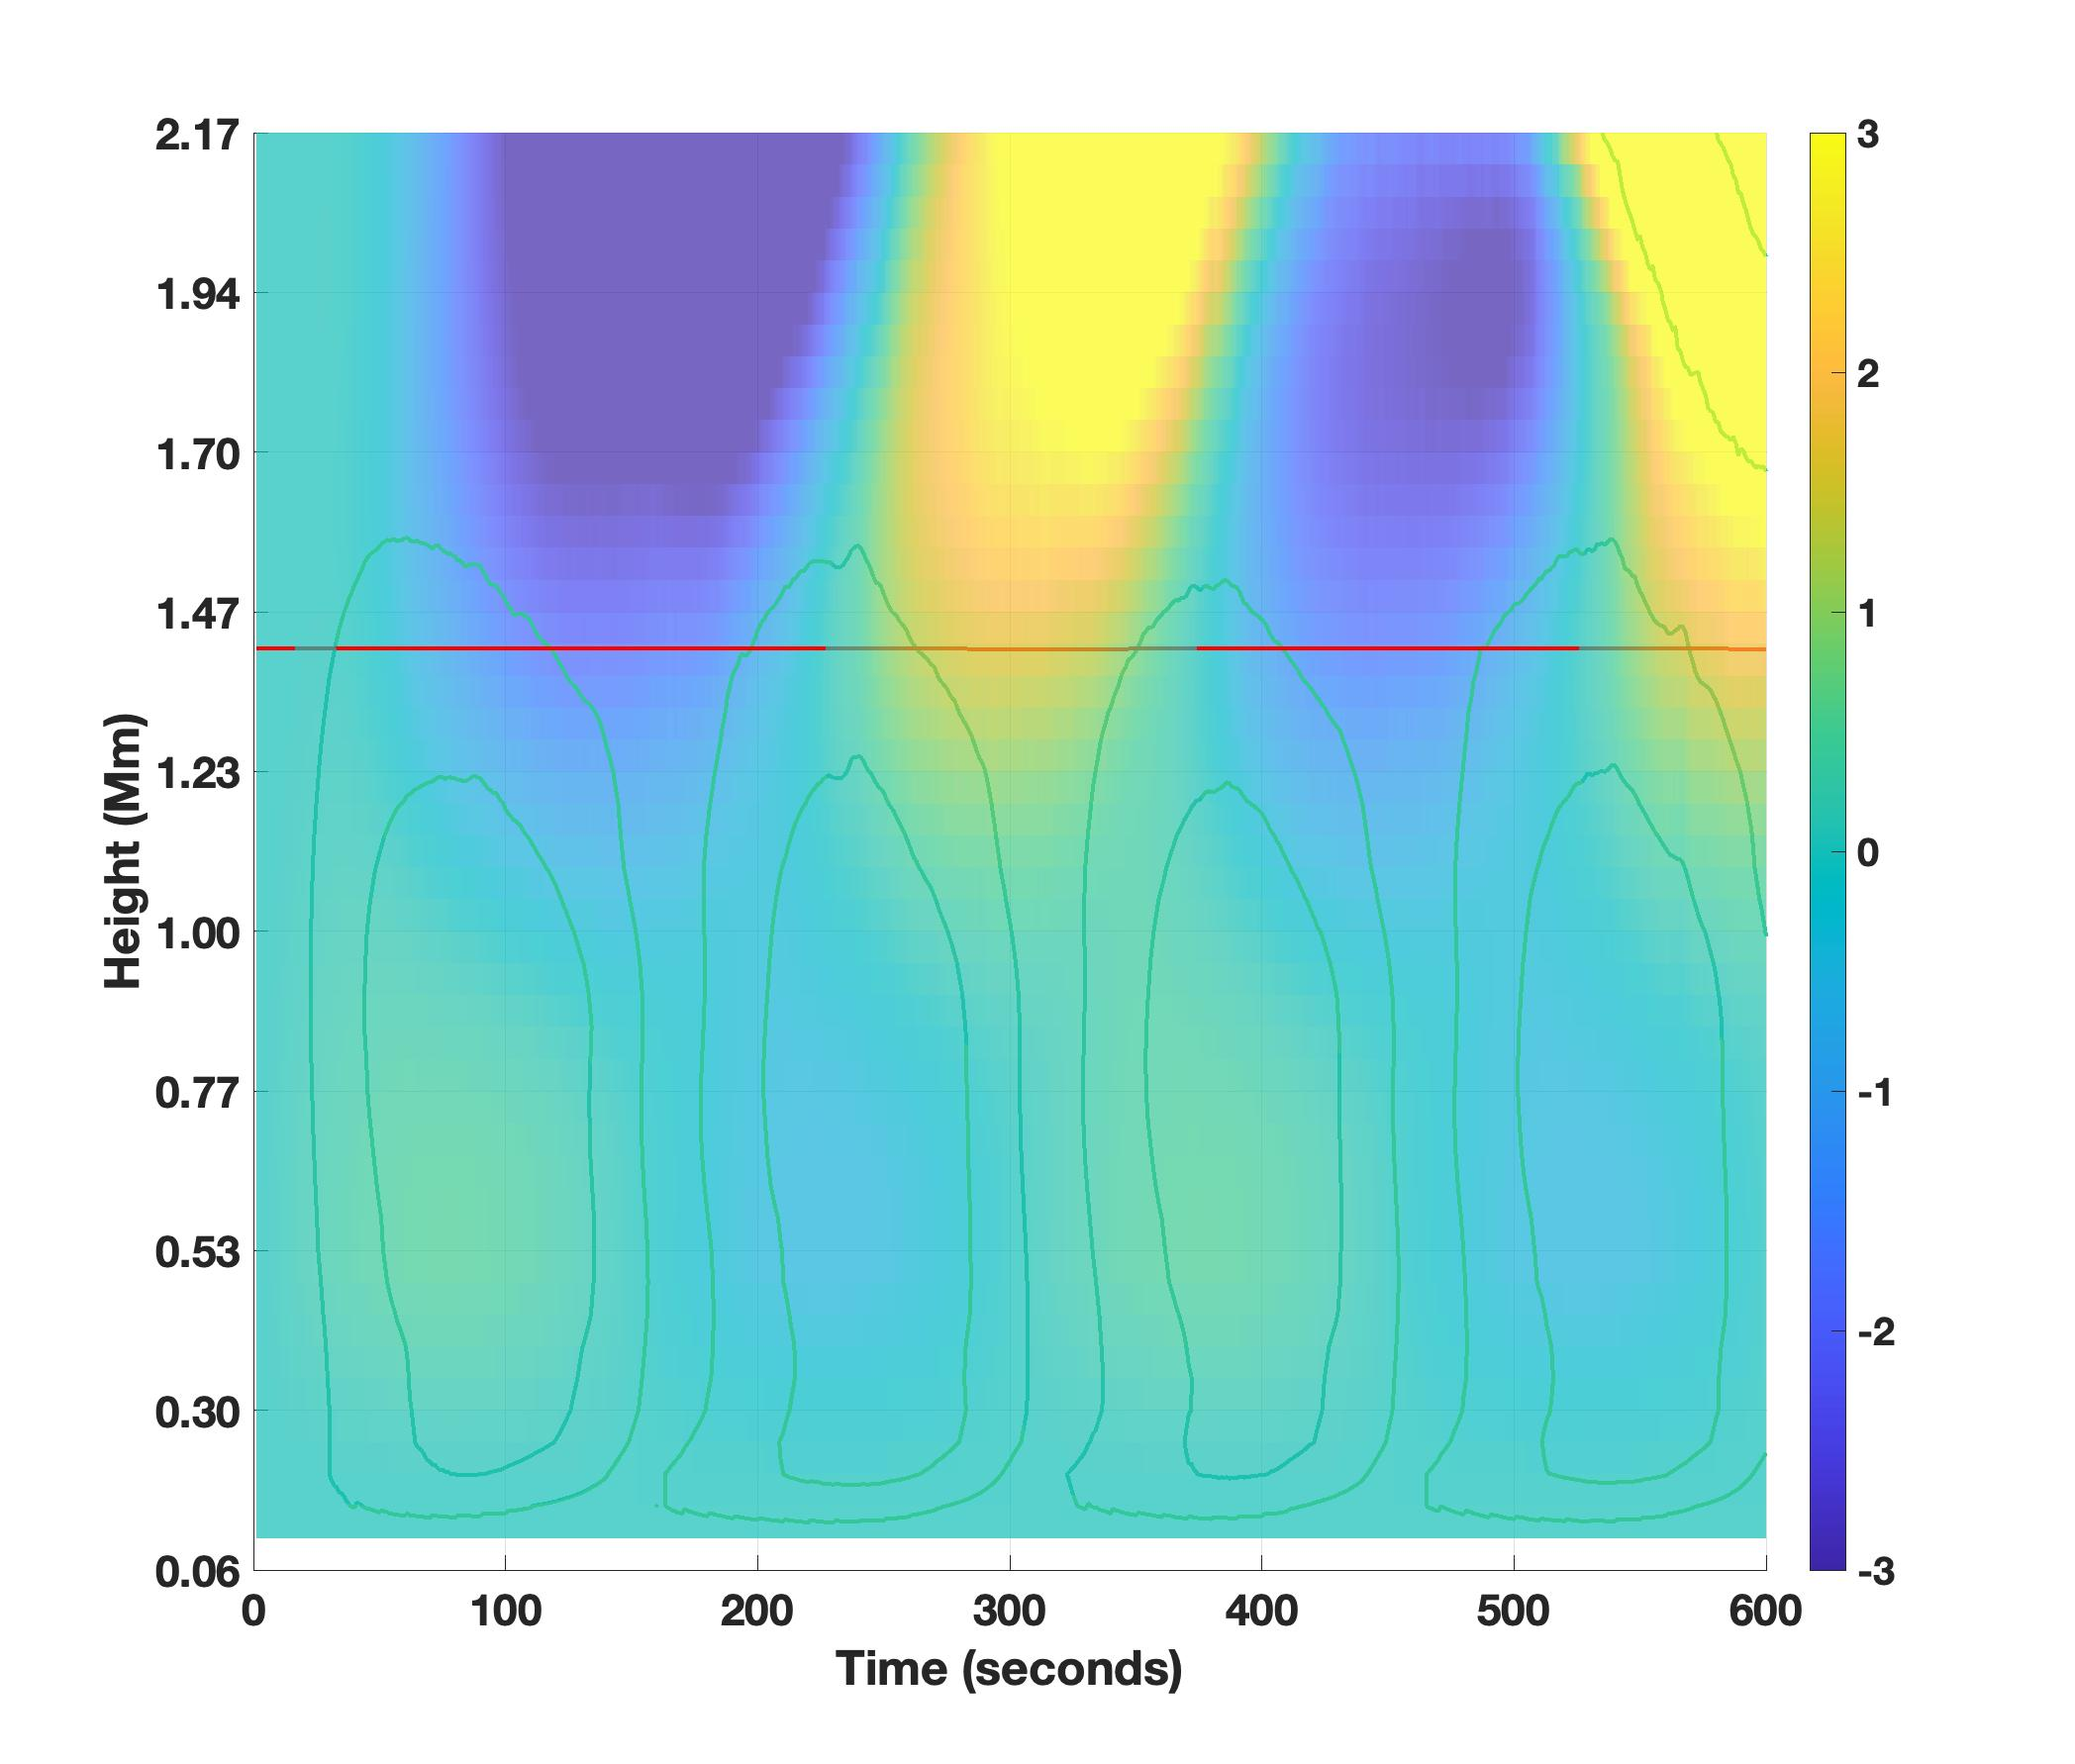
\includegraphics[scale=0.25]{td_vert_bv100G_300_with_bandbeta.jpg}
\caption{Distance-time plot of the vertical component of the velocity in the mid chromosphere, for the case with magnetic field of 100G, showing  contours for the perturbed magnetic field, the horizontal lines are contours for the plasma beta. The lower, middle and upper lines correspond to values for the plasma beta of 50, 0.97 and 0.5 respectively.}
%\caption{Energy Flux for the mid-section of the Simulation for 76s, 150s, 225s and 330s for a vertical field with maximum field of 50G }
\end{figure}

\begin{figure}
\centering
\label{td_vert_dif_bv0G_100G_300}
%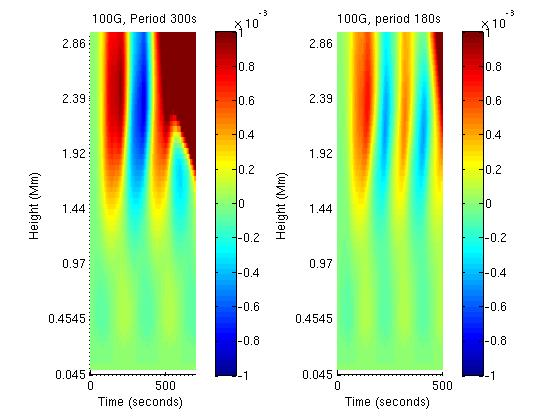
\includegraphics[scale=0.475]{dt_vvert_100G_300s_180s.jpg}
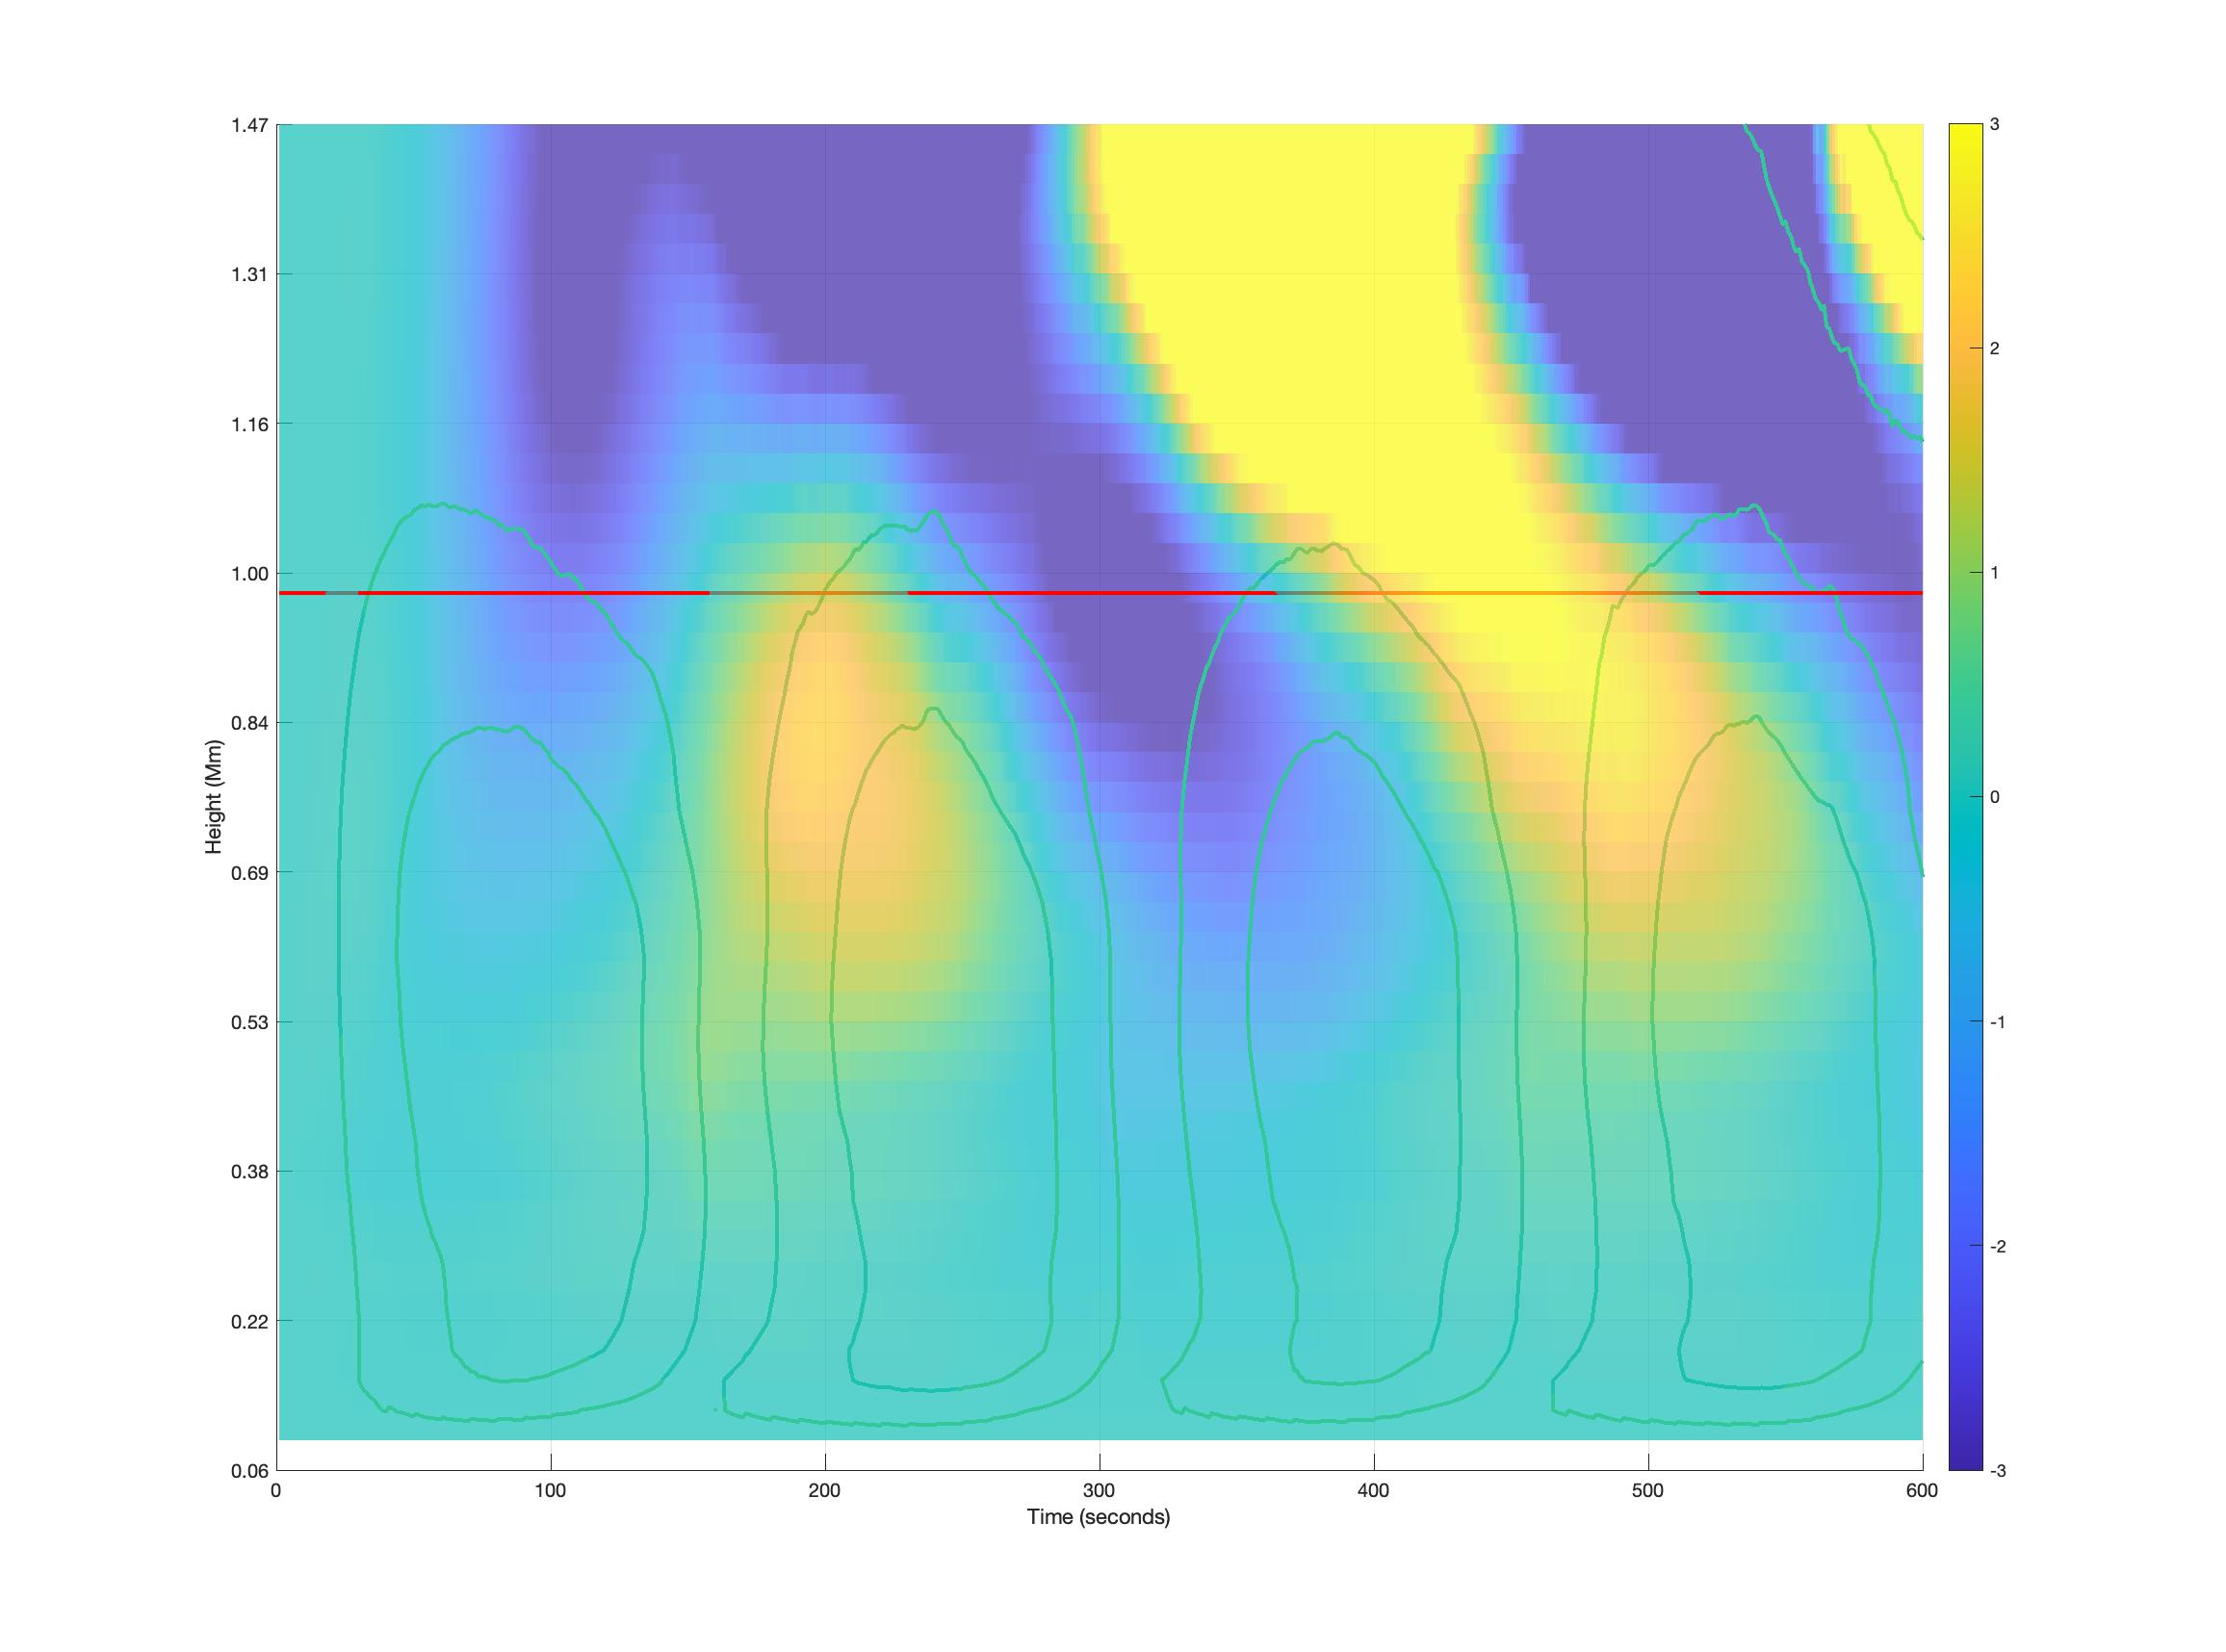
\includegraphics[scale=0.3]{td_vert_dif_bv0G_100G_300.jpg}
\caption{Distance-time plot of the vertical component of the velocity in the mid chromosphere, for the case of the difference between 0G and 100G, showing the line of beta equal to 0.97 and contours for the perturbed magnetic field}
%\caption{Energy Flux for the mid-section of the Simulation for 76s, 150s, 225s and 330s for a vertical field with maximum field of 50G }
\end{figure}


To investigate the influence of the magnetic field on the propagation of wave energy we employ an expression for the energy flux which was used by \citet{Bogdan2003}. The wave energy flux $\bf{F}_{wave}$ is given by
$$
{\mathbf F}_{wave}=\tilde{p}_{k} {\mathbf v}+\tilde{\mathbf B}\cdot {\mathbf B_{b}}{\mathbf v}+{\mathbf v}\cdot \tilde{\mathbf B}{\mathbf B_{b}} .
$$

We compute the time averaged energy flux integrated over different cross sections of the simulation box.

\begin{equation}
F_{int}= \frac{1}{t_{max}} \int_{0}^{t_{max}} \int {\mathbf F}_{wave} \cdot d{\mathbf A}dt,
\label{e11}
\end{equation}

These expression are dependent on the perturbed kinetic pressure $\tilde{p}_{k}$.
$$
\tilde{p}_{k}=\left(\gamma - 1\right)\left( \tilde{e}-\frac{ \left( \tilde{\rho} +\rho_b \right){\mathbf v}^2}{2}-\frac{{\mathbf B}^2}{2}\right).
$$
Using equation (\ref{e11}), we computed the energy flux integral for each of the drivers at different atmospheric heights and averaged over the total time. We compute the ratio of this integrated energy flux to the integrated energy flux at the location of the driver, the resulting values are shown in table 2 . It appears that for heights greater than 4Mm, the energy flux is enhanced for increasing values for the vertical magnetic field. In figure \ref{energyfluxratio_50G_75G_100G_line},  we plot the ratio of the integrated energy flux ratio for different values of the field at different heights and for the different vertical field values ( the blue, orange and red  are for field values of 50G, 75G and 100G respectively). This plot demonstrates that for higher B-field magnitudes there is a small leakage of energy propagation, this is interesting because this is consistent with observations and other simulation results which demonstrate an enhancement for inclined fields.


%% \ref{energyfluxratio_50G_75G_100G_line}. figure 5 above
%%\ref{energyflux}

%%ratios for two sets of simulations. In the first case we show the energy flux ratios for our drivers each delivering the same amount of energy, in the second case (figure 
%\ref{Fig19}
%%), we plot the energy ratios for another set of simulations but where we kept the driver amplitude fixed at the same amplitude for all mode numbers and driver frequencies. The energy flux ratio is the ratio of the energy flux at a given height to the energy flux at the location of the driver. 

\begin{figure}
    \label{energyfluxratio_50G_75G_100G_line}
    \centering
    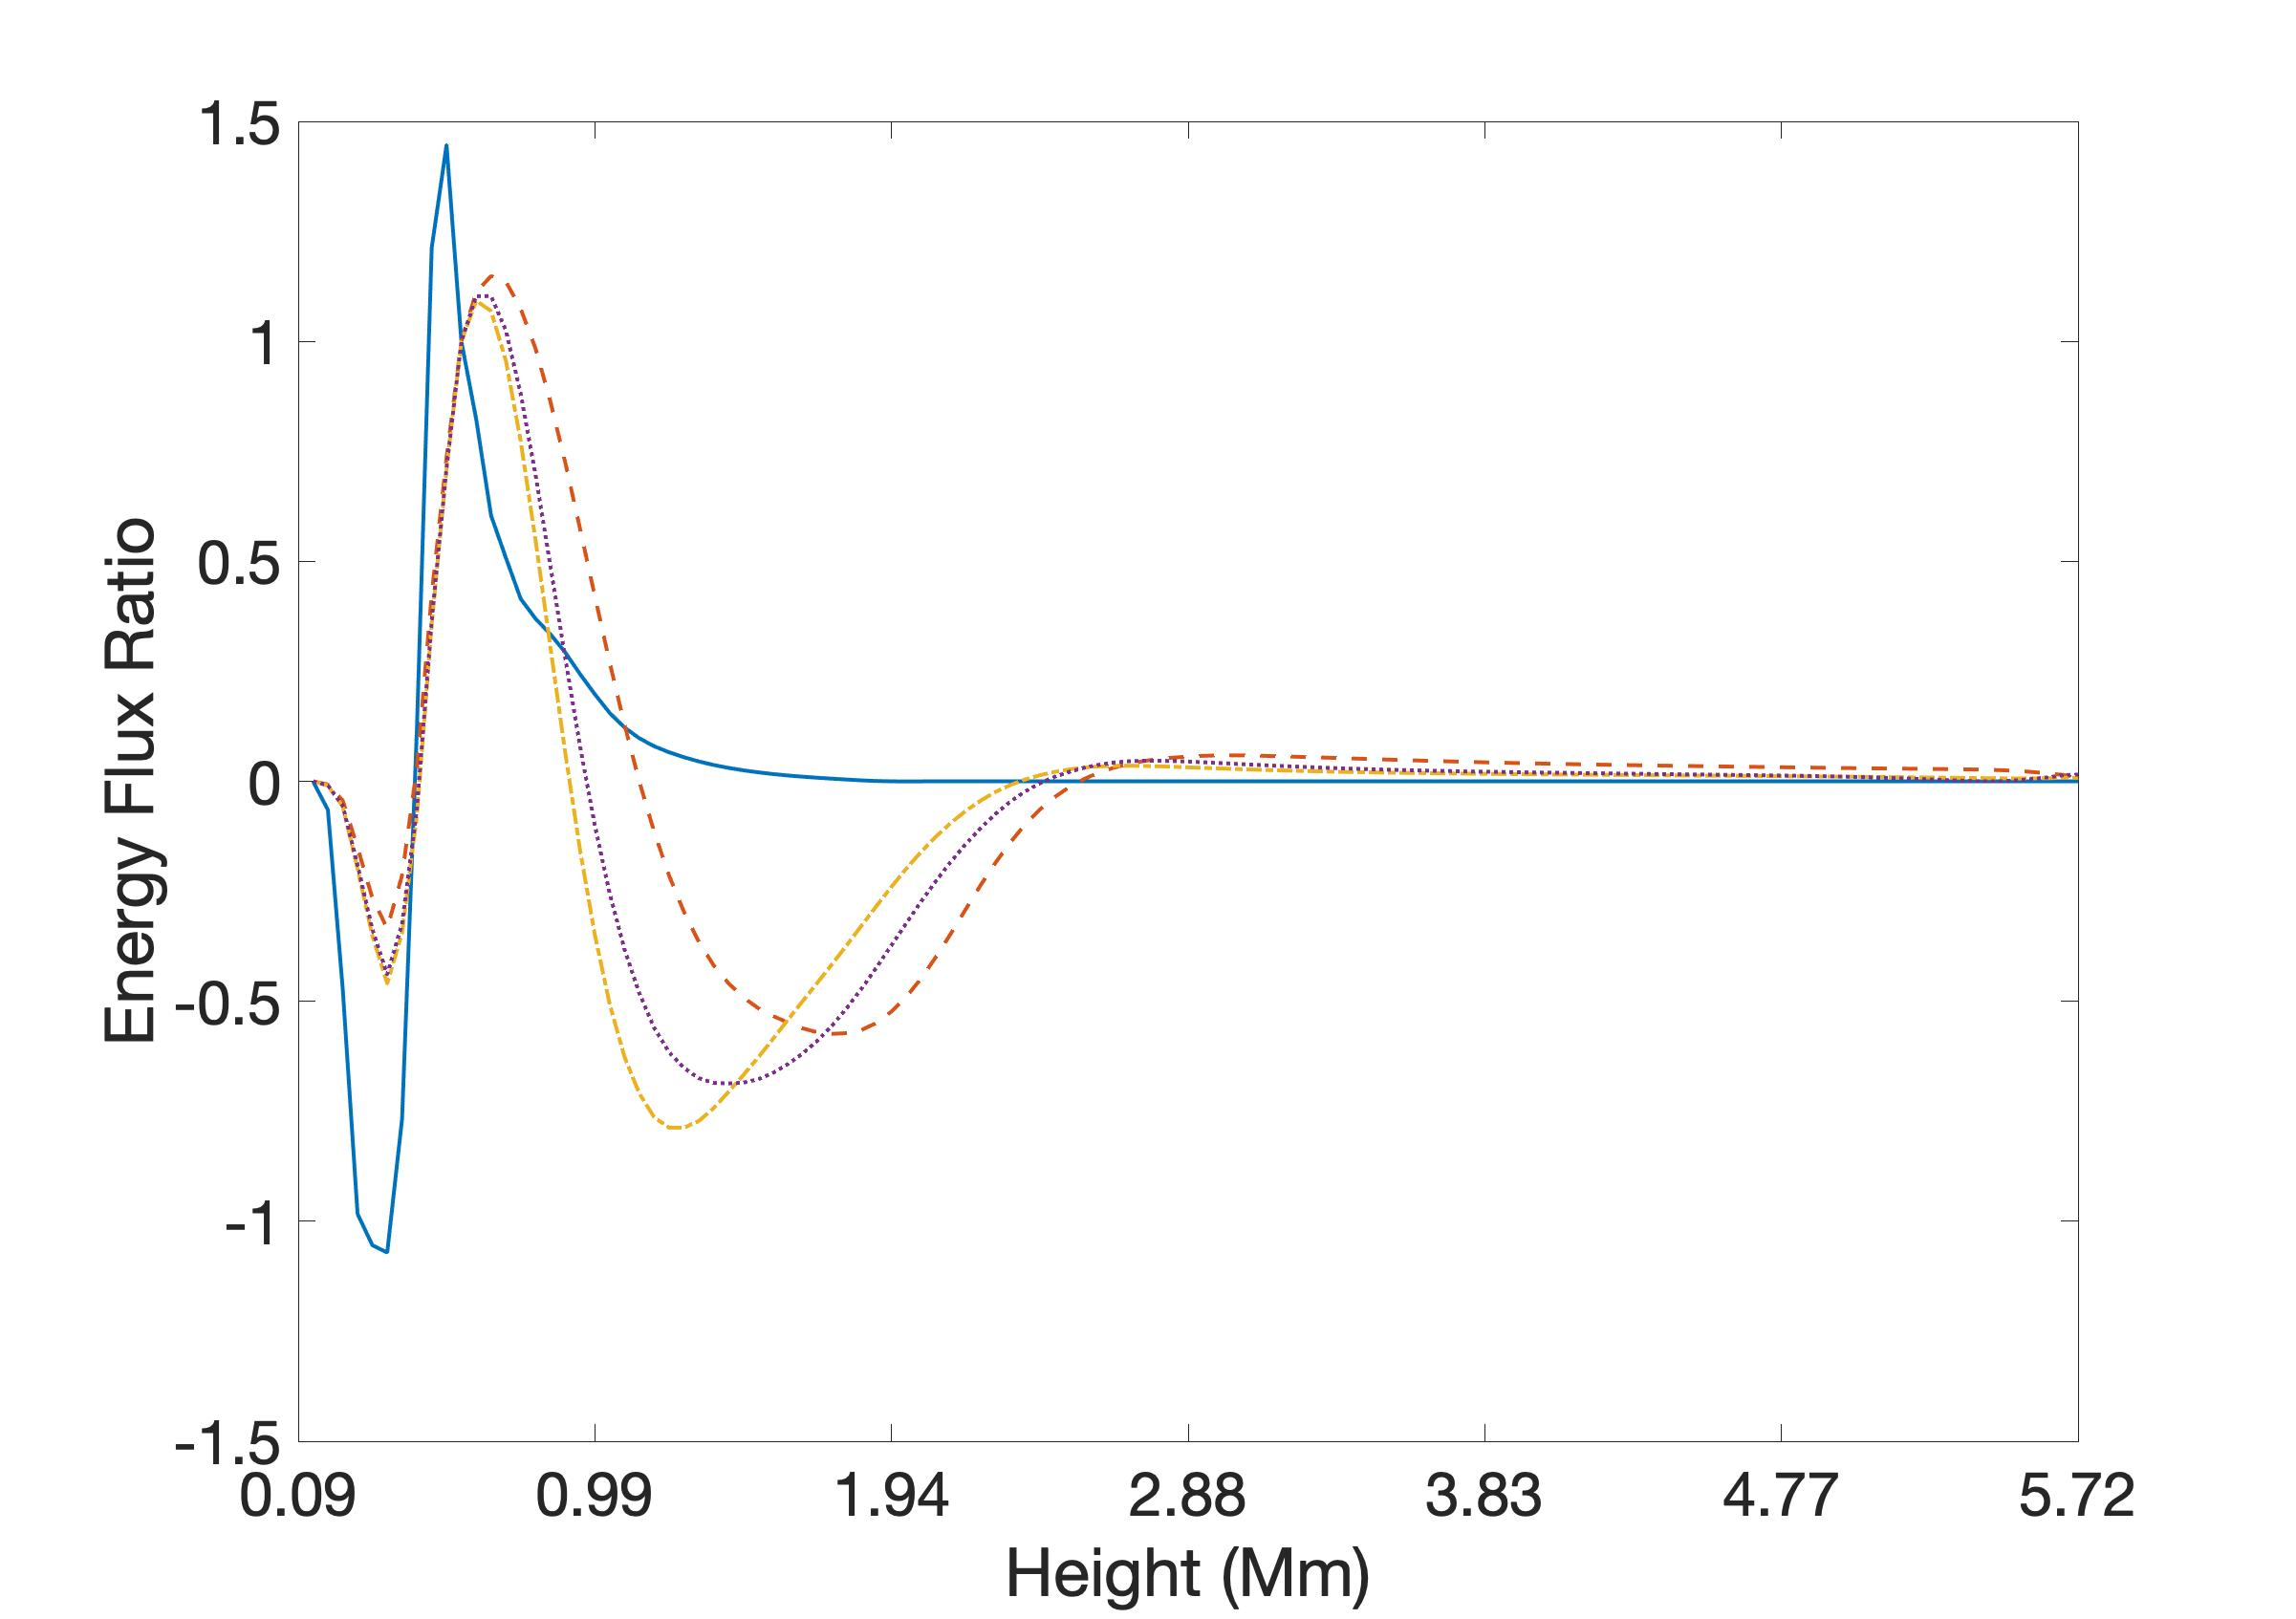
\includegraphics[scale=0.2]{energyfluxratio.jpg}
    \caption{Shows the Ratio of the Integrated Energy Flux ratio for different values of the field, Blue 50G, Orange 75G, Red 100GMm}
\end{figure}

\begin{figure}
    \centering
    \label{fft_sim}
    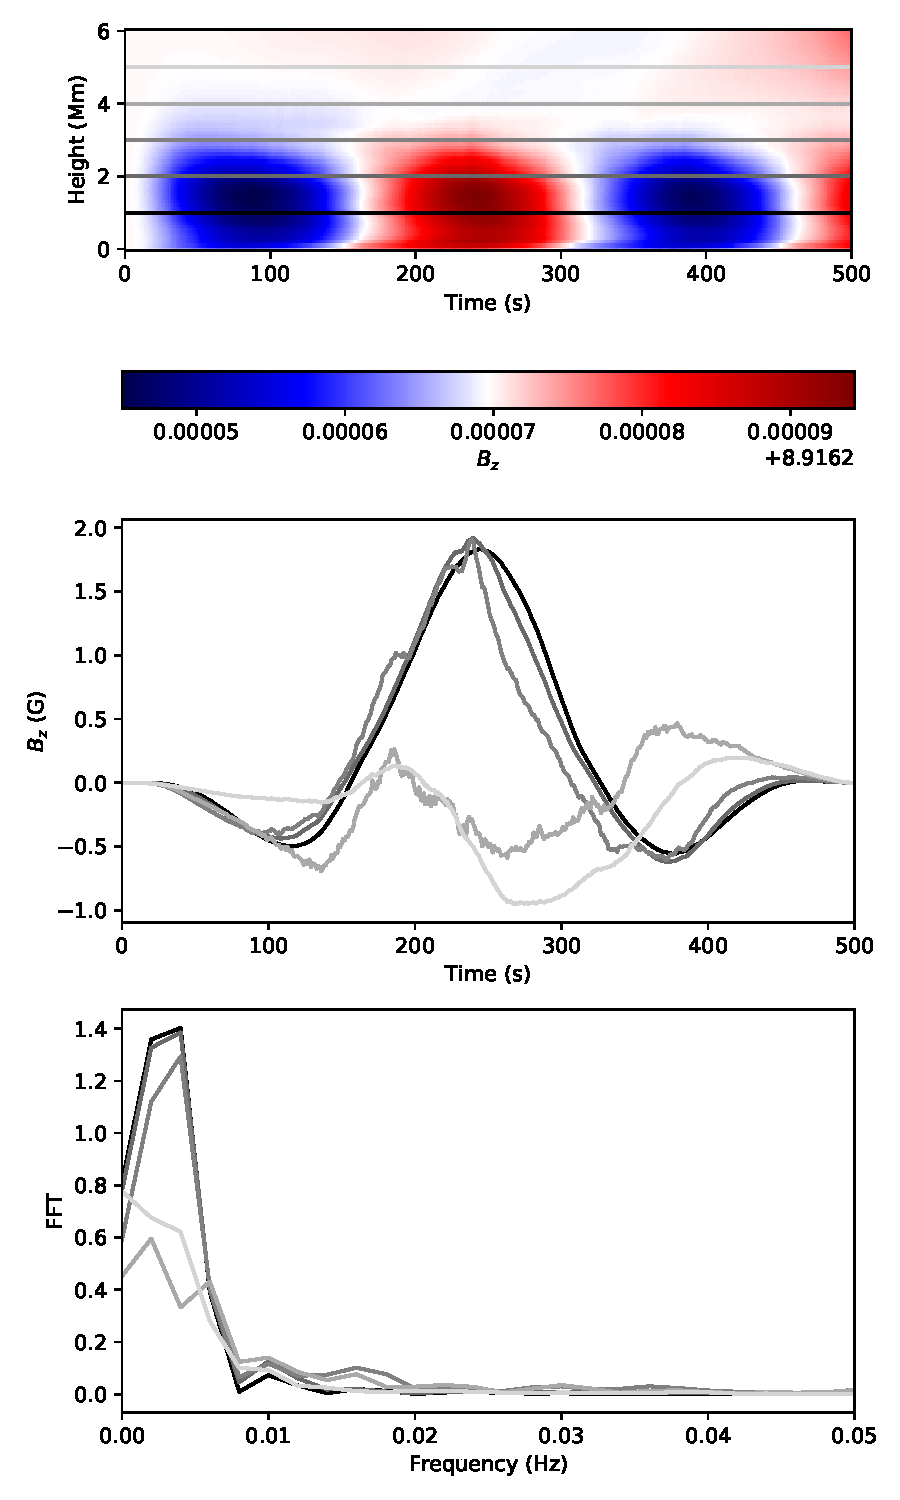
\includegraphics[scale=0.55]{fft_sim.pdf}
    \caption{Temporal analysis of $Bz$ vertical slices at $2$ $Mm$. The top panel shows the selected vertical slices, indicated by gray colours. The middle panel demostrates the obtained signal after applying a Hanning window function. The bottom panel shows the result of the FFT analysis based on the $5$ selected vertical $Bz$ slices.}

    \centering
    \label{fft_sim}
    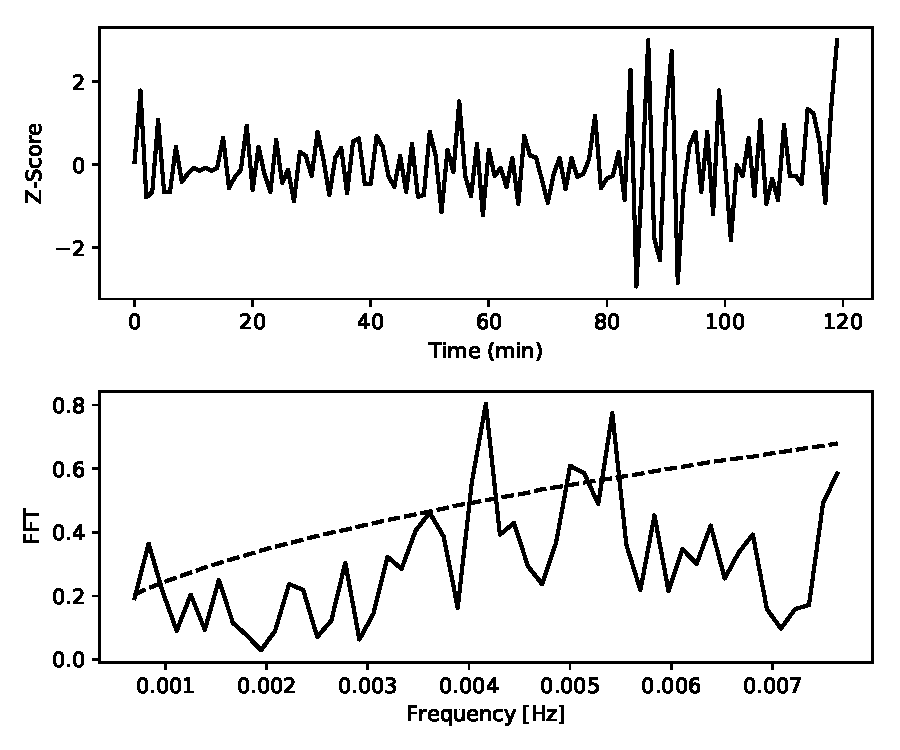
\includegraphics[scale=0.55]{fft_obs.pdf}
    \caption{Temporal analysis of pixel intensity based on AIA 1600{\AA} between 18:00 UT to 20:00 UT on 22 August 2010. The upper panel shows the temporal variation of the Z-Score (detrended and normalised pixel intensity data). The lower panel shows the FFT of the analysed observational data. }
\end{figure}

\begin{figure}
    \label{obs}
    \centering
    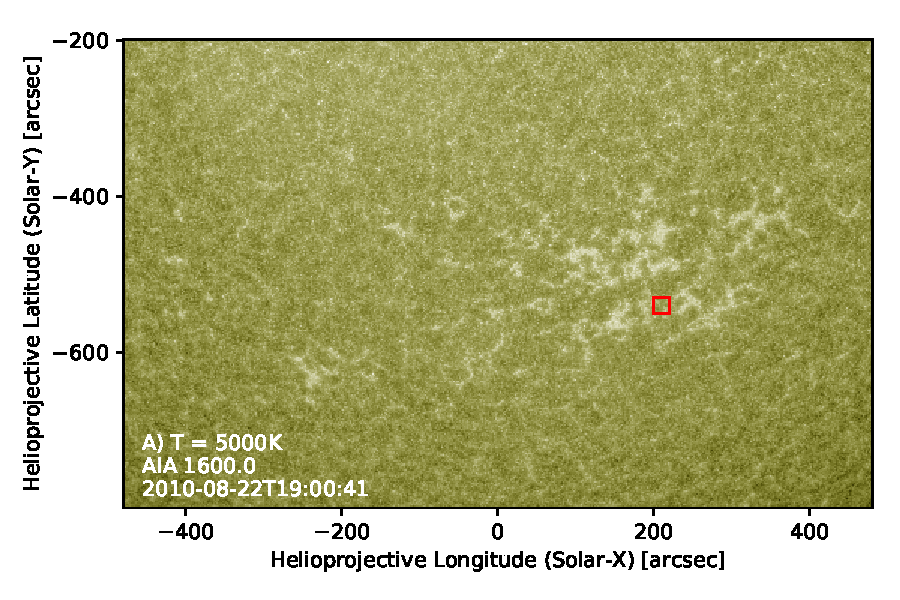
\includegraphics[scale=0.5]{obs_data.pdf}
    \caption{The selected pixel from the start of the investigate time series at 18:00 UT on 22 August 2010. The pixel is indicated by red rectangle.}
\end{figure}

\section{Frequency Analysis}

The top panel of Figure \ref{fft_sim} shows a vertical slice of $Bz$ over time, this is based on the simulation with the initial magnetic field configuration with a maximum value of $100$G. The vertical axis represents the height in Mm and the horizontal axis is the time dimension, measured in seconds. From this 2-dimensional plane, we selected $5$ layers, indicated by vertical grey lines. The middle panel of Figure \ref{fft_sim} displays the temporal variation of the selected layers, indicated by different grey shade colours. The time series do not feature non-stationary behaviour, therefore, further transformations (such as de-trending, smoothing or differentiation) are not needed. The Hanning-window function is still applied to avoid leakage effects when performing the Fast Fourier Transformation (FFT).  

An FFT is applied (the lower panel) for investigating any oscillatory behaviour in the analysed signal. A significant oscillatory pattern is found with frequency range of $3.75$ - $4$mHz , corresponding a period range of $4.2$ - $4.4$ minutes. FFT was also performed based on other simulations with different initial magnetic field configurations (with a maximum value of $0$G , $50$G  $75$G  and $100$G ). These investigations all showed similar oscillatory behaviour, therefore, we present one FFT as a representative example. 

Next, temporal analysis for observational data is performed for confirming the obtained oscillatory behaviour. We investigate intensity oscillations in the solar atmosphere observed by SDO/AIA. The passband 1600 {\AA} is selected because our simulation mainly focuses on lower atmospheric regions, i.e. photosphere and chromosphere. The cadence of 1600 {\AA} images is 24 seconds, therefore it is suitable for studying relatively high-frequency oscillations such as the obtained $4$mHz.

The initial magnetic field configuration of our model is a standing magnetic tube, passing through the chromosphere and the lower corona. Therefore, We chose to sample a typical active region. The selected area contains a small sunspot (solar pore), presumably featuring similar magnetic structure as our simulation. From each observation, a single pixel is selected, yielding a $0.35$Mm  by $0.35$Mm  area. The obtained time series shows non-stationary behaviour, therefore, the observed linear trend is removed by taking the first difference $\Delta  y_{t}$ of the data. The first difference is defined as the difference between consecutive observations $y_{t}$ and $y_{t-1}$. Furthermore, the times series is also normalised by applying standard scores (Z-scores), defined by:

\begin{equation}
	Z_{i} = \frac {T_{i} - \overline{T}}  {\sigma(T)},
	\label{z_score}
\end{equation}

where, the parameter $\overline{T}$ is the mean of the time series and the parameter $\sigma(T)$ is defined as the standard deviation of the data. The top panel of Figure \ref{fft_sim} demonstrates the trend removed and normalised time series. The lower panel of Figure \ref{fft_sim} shows the result of the applied FFT technique. The dashed line is the significance level ($3 \sigma$) which is calculated by Monte-Carlo method. The original data showed red noise signature which transformed to blue noise after differentiating the data. We have generated 1 million blue noise signatures $N_{b}$ and calculated the standard deviation $\sigma(N_{b})$ and the mean $\overline{N_{b}}$ of the simulated noise, providing our significance level $S$:

\begin{equation}
    S = \overline{N_{b}} + 3 \sigma(N_{b}).
\end{equation}

A significant period is found with frequency range of $4-4.2$mHz , corresponding a period range of $4$ - $4.2$ minutes, which is close to the period found in simulation data. Another significant peak is found with period around $3$ minutes which may be an indication of another global oscillation.

\section{Conclusion}


{\bcr A number of helioseismic studies have shown that high frequency pmodes can leak into the upper atmosphere (though are evanescent) without magnetic fields. Comparing quiet sun and magnetic observations is vital before you make any connections with the model. Finally, the authors conclude that their spectral analysis shows a larger shift than whats been previously observed by hindman et al. 1996, but then state that this is explained in part by the work of Campbell and Roberts 1989. Campbell and Roberts state very different behavior depending on the radial order $n$ and harmonic degree $\ell$. If the observed frequency shift is consistent with what Campbell and Roberts find, the authors should explain why. Is it because your source term emulates certain ell and n modes. What happens with your spectral results when you change the source term. A meaningful discussion is required here if the reader is to gain any insight into the physics at play.

}


In this paper we have presented results for a series of MHD simulations of an extended oscillator at the base of a model solar atmosphere. We have shown that energy is propagated by magnetosonic modes. Slow and fast magnetosonic modes are responsible for carrying some energy back to the chromosphere and the photosphere. The results exhibit a small frequency shift  for different values of the magnetic field closer inspection of the energy flux propagation results indicative of enhanced energy flux propagation for inclined magnetic fields. The obtained periodic behaviour is confirmed by observational data, featuring similar frequencies based on the intensity times series of SDO images. The frequency shift measured from the temporal analysis of the observational and simulation data is larger than would be expected from the analysis of \citet{Hindman1996}. This can be understood in part by referring to the work of \citet{Campbell1989}.


It is encouraging that the results presented here are consistent with the behaviour exhibited  by earlier work. Significant improvements to the comparisons presented in this paper are expected with the  recent work of \citet{Kostogryz2021}. Here modelling of intensity perturbations using a VALIIIc solar atmosphere model with radiative transfer the intensity oscillations perturbed by the solar global oscillations modelled using the ADIPLS code of \citet{Christensen-Dalsgaard2008}. Also, as described in \citet{Rast2016}, more sensitive observations with instruments such as DKIST may enable further constraints and the range of theoretical models. Future work will address simulation runs over longer time periods and for inclined fields. There is an issue that due to the extended nature of the driver the amplitudes used may be responsible for delivering vast quantities of energy into the solar atmosphere and for driving a highly numerically unstable system and inducing extremely large shocks \citet{Santamaria2015}. 
%e.g. cite reference Solar Physics Fedun et al 2009 oscillatory response 3d solar atmosphere to leakage of photospheric motions

%% If you wish to include an acknowledgments section in your paper,
%% separate it off from the body of the text using the \acknowledgments
%% command.

\section{Acknowledgments}
%\acknowledgments

The authors thank P. H. Keys for providing the wavelet tools to analyse the related SDO data M.Korsos for the preparation of Figure 1, the Science and Technology Facilities Council (STFC) for the support they received.  RE acknowledges the support received from the the Royal Society (UK). We acknowledge IT Services at The University of Sheffield for the provision of the High Performance Computing Service.


%% To help institutions obtain information on the effectiveness of their 
%% telescopes the AAS Journals has created a group of keywords for telescope 
%% facilities.
%
%% Following the acknowledgments section, use the following syntax and the
%% \facility{} or \facilities{} macros to list the keywords of facilities used 
%% in the research for the paper.  Each keyword is check against the master 
%% list during copy editing.  Individual instruments can be provided in 
%% parentheses, after the keyword, but they are not verified.

%%\vspace{5mm}
%%\facilities{HST(STIS), Swift(XRT and UVOT), AAVSO, CTIO:1.3m,
%%CTIO:1.5m,CXO}

%% Similar to \facility{}, there is the optional \software command to allow 
%% authors a place to specify which programs were used during the creation of 
%% the manusscript. Authors should list each code and include either a
%% citation or url to the code inside ()s when available.

\software{SMAUG \citet{Griffiths2015}, SAC \citet{Shelyag2008},             
          VAC \citet{Toth1996}
          }

%% Appendix material should be preceded with a single \appendix command.
%% There should be a \section command for each appendix. Mark appendix
%% subsections with the same markup you use in the main body of the paper.

%% Each Appendix (indicated with \section) will be lettered A, B, C, etc.
%% The equation counter will reset when it encounters the \appendix
%% command and will number appendix equations (A1), (A2), etc. The
%% Figure and Table counter will not reset.

%%\appendix



%% The reference list follows the main body and any appendices.
%% Use LaTeX's thebibliography environment to mark up your reference list.
%% Note \begin{thebibliography} is followed by an empty set of
%% curly braces.  If you forget this, LaTeX will generate the error
%% "Perhaps a missing \item?".
%%
%% thebibliography produces citations in the text using \bibitem-\cite
%% cross-referencing. Each reference is preceded by a
%% \bibitem command that defines in curly braces the KEY that corresponds
%% to the KEY in the \cite commands (see the first section above).
%% Make sure that you provide a unique KEY for every \bibitem or else the
%% paper will not LaTeX. The square brackets should contain
%% the citation text that LaTeX will insert in
%% place of the \cite commands.

%% We have used macros to produce journal name abbreviations.
%% \aastex provides a number of these for the more frequently-cited journals.
%% See the Author Guide for a list of them.

%% Note that the style of the \bibitem labels (in []) is slightly
%% different from previous examples.  The natbib system solves a host
%% of citation expression problems, but it is necessary to clearly
%% delimit the year from the author name used in the citation.
%% See the natbib documentation for more details and options.

\begin{thebibliography}{}


\bibitem[{{Bogdan} et~al.(2003){Bogdan}, {Carlsson}, {Hansteen}, {McMurry},
  {Rosenthal}, {Johnson}, {Petty-Powell}, {Zita}, {Stein}, {McIntosh}, and
  {Nordlund}}]{Bogdan2003}
{Bogdan}, T.~J., {Carlsson}, M., {Hansteen}, V.~H., {McMurry}, A., {Rosenthal},
  C.~S., {Johnson}, M., {Petty-Powell}, S., {Zita}, E.~J., {Stein}, R.~F.,
  {McIntosh}, S.~W., {Nordlund}, {\AA}., 2003. {Waves in the Magnetized Solar
  Atmosphere. II. Waves from Localized Sources in Magnetic Flux
  Concentrations}. \apj 599, 626--660.

\bibitem[{{Calvo Santamaria}, {Khomenko} and {Collados}  (2015)}]{Santamaria2015}
 {Calvo Santamaria}, I., {Khomenko}, E.,  and {Collados}, M., 2015. {Magnetohydrodynamic wave propagation from the subphotosphere to the corona in an arcade-shaped magnetic field with a null point}. \aap 577, A70.


\bibitem[{{Campbell} and {Roberts} (1989)}]{Campbell1989}
 {Campbell}, W.~R. and {Roberts}, B.\ 1989. {The Influence of a Chromospheric Magnetic Field on the Solar p- and f-Modes} \apj, 338, 538. doi:10.1086/167216

\bibitem[{{Carlsson} and {Stein}(1995)}]{Carlsson1995}
{Carlsson}, M., {Stein}, R.~F., 1995. {Does a nonmagnetic solar chromosphere
  exist?} \apjl 440, L29--L32.

\bibitem[{{Caunt} and {Korpi}(2001)}]{Caunt2001}
{Caunt}, S.~E., {Korpi}, M.~J., Apr. 2001. A {3D} {MHD} model of astrophysical
  flows: Algorithms, tests and parallelisation. \aap 369, 706--728.

\bibitem[Christensen-Dalsgaard(2008)]{Christensen-Dalsgaard2008} Christensen-Dalsgaard, J.\ 2008, \apss, 316, 113. doi:10.1007/s10509-007-9689-z


\bibitem[Edwin \& Roberts(1983)]{EdwinandRoberts1983} Edwin, P.~M. \& Roberts, B.\ 1983, \solphys, 88, 179. doi:10.1007/BF00196186

\bibitem[Erd{\'e}lyi(2006)]{Erdelyi2006} Erd{\'e}lyi, R.\ 2006, Philosophical Transactions of the Royal Society of London Series A, 364, 351. doi:10.1098/rsta.2005.1703

\bibitem[{{Fedun} et~al.(2009a){Fedun}, {Erd{\'e}lyi}, and
  {Shelyag}}]{Fedun2009a}
{Fedun}, V., {Erd{\'e}lyi}, R., {Shelyag}, S., Sep. 2009. {Oscillatory Response
  of the 3D Solar Atmosphere to the Leakage of Photospheric Motion}. \solphys
  258, 219--241.

\bibitem[{{Fedun} et~al.(2009b){Fedun}, {Erd{\'e}lyi}, and
  {Shelyag}}]{Fedun2009b}
{Fedun}, V., {Erd{\'e}lyi}, R., {Shelyag}, S., Sep. 2009. {MHD waves generated by high-frequency photospheric vortex motions}. Annales Geophysicae
  29, 1029-1035.

\bibitem[{{Griffiths} et~al.(2015){Griffiths}, {Fedun}, and
  {Erd{\'e}lyi}}]{Griffiths2015}
{Griffiths}, M.~K., {Fedun}, V., {Erd{\'e}lyi}, R., 2015. {A Fast MHD Code for
  Gravitationally Stratified Media using Graphical Processing Units: SMAUG}.
  Journal of Astrophysics and Astronomy 36, 197--223.

\bibitem[{{Griffiths} et~al.(2017){Griffiths}, {Erd{\'e}lyi}, and
  {Fedun}}]{Griffiths2017}
{Griffiths}, M., {Erd{\'e}lyi}, R., {Fedun}, V., 2017. {Videos of
  Magnetohydrodynamics Simulations of Solar Atmosphere Wave Dynamics Generated
  by Solar Global Oscillating Eigenmodes}.
\newline \url{https://figshare.com/articles/Videos_of_Magnetohydrodynamics_Simulations_of_Solar_Atmosphere_Wave_Dynamics_Generated_by_Solar_Global_Oscillating_Eigenmodes/4818490}

\bibitem[{{Griffiths} et~al.(2018a){Griffiths2018a}, {Erd{\'e}lyi}}]{Griffiths2018a}
{Griffiths}, M., {Erd{\'e}lyi}, R., {Fedun}, V., 2018. {Videos of p-Mode Oscillations in Highly Gravitationally Stratified Magnetic Solar Atmospheres}.
\newline \url{https://figshare.shef.ac.uk/articles/dataset/Videos_of_p-Mode_Oscillations_in_Highly_Gravitationally_Stratified_Magnetic_Solar_Atmospheres/7378046}




\bibitem[{{Griffiths} et~al.(2018b)}]{Griffiths2018b}
{Griffiths}, M.~K., {Fedun}, V., {Erd{\'e}lyi}, R., and {Zheng},R.,
{Solar atmosphere wave dynamics generated by solar global oscillating
  eigenmodes}.{Advances in Space Research}, 61: 720--737, January 2018.

\bibitem[{Gudiksen} et~al.(2011){Gudiksen}, {Carlsson}, {Hansteen}, {Hayek},
  {Leenaarts}, and {Mart{\'{\i}}nez-Sykora}]{Gudiksen2011}
B.~V. {Gudiksen}, M.~{Carlsson}, V.~H. {Hansteen}, W.~{Hayek}, J.~{Leenaarts},
  and J.~{Mart{\'{\i}}nez-Sykora}.
\newblock {The stellar atmosphere simulation code Bifrost. Code description and
  validation}.
\newblock \emph{\aap}, 531:\penalty0 A154, July 2011.
\newblock \doi{10.1051/0004-6361/201116520}.


\bibitem[Hasan \& Christensen-Dalsgaard(1992)]{Hasan1992} Hasan, S.~S. \& Christensen-Dalsgaard, J.\ 1992, \apj, 396, 311. doi:10.1086/171718



\bibitem[{{Hindman} et~al.(1996)}]{Hindman1996}
{Hindman}, B.~W. and {Zweibel}, E.~G. and {Cally}, P.~S., Mar. 1996. {Driven Acoustic Oscillations within a Vertical Magnetic Field}. \apj 459, 760--772.

\bibitem[{{Kalkofen}(2012)}]{Kalkofen2012}
{Kalkofen}, W., 2012. {The Validity of Dynamical Models of the Solar
  Atmosphere}. \solphys 276, 75--95.

\bibitem[{{Khomenko} and {Calvo Santamaria}(2013)}]{Khomenko2013}
{Khomenko}, E., {Calvo Santamaria}, I., 2013. {Magnetohydrodynamic waves driven
  by p-modes}. Journal of Physics Conference Series 440~(1), 012048.


\bibitem[{Kontogiannis} et~al.(2010){Kontogiannis}, {Tsiropoula}, and
  {Tziotziou}]{Kontogiannis2010}
I.~{Kontogiannis}, G.~{Tsiropoula}, and K.~{Tziotziou}.
\newblock {Power halo and magnetic shadow in a solar quiet region observed in
  the H{$\alpha$} line}.
\newblock \emph{\aap}, 510:\penalty0 A41, February 2010.
\newblock \doi{10.1051/0004-6361/200912841}.

\bibitem[Kostogryz et al.(2021)]{Kostogryz2021} Kostogryz, N.~M., Fournier, D., \& Gizon, L.\ 2021, \aap, 654, A1. doi:10.1051/0004-6361/202040264



\bibitem[{{Leenaarts} et~al.(2011){Leenaarts}, {Carlsson}, {Hansteen}, and
  {Gudiksen}}]{Leenaarts2011}
{Leenaarts}, J., {Carlsson}, M., {Hansteen}, V., {Gudiksen}, B.~V., 2011. {On
  the minimum temperature of the quiet solar chromosphere}. \aap 530, A124.


\bibitem[{{Leighton}(1960)}]{Leighton1960}
{Leighton}, R.~B., 1960. In: {Thomas}, R.~N. (Ed.), Aerodynamic Phenomena in
  Stellar Atmospheres. Vol.~12 of IAU Symposium. pp. 321--325.

\bibitem[{{Malins}(2007)}]{Malins2007}
{Malins}, C., 2007. {On transition region convection cells in simulations of
  $\{$p$\}$-mode propagation}. Astronomische Nachrichten 328, 752--755.


\bibitem[{{McWhirter} et~al.(1975){McWhirter}, {Thonemann}, and
  {Wilson}}]{McWhirter1975}
{McWhirter}, R.~W.~P., {Thonemann}, P.~C., {Wilson}, R., 1975. {The heating of
  the solar corona. II - A model based on energy balance}. \aap 40, 63--73.

\bibitem[{{Murawski} and {Zaqarashvili}(2010)}]{Murawski2010}
{Murawski}, K., {Zaqarashvili}, T.~V., 2010. {Numerical simulations of spicule
  formation in the solar atmosphere}. \aap 519, 9.

\bibitem[Pint{\'e}r et al.(2007)]{Pinter2007} Pint{\'e}r, B., Erd{\'e}lyi, R., \& Goossens, M.\ 2007, \aap, 466, 377. doi:10.1051/0004-6361:20041632

\bibitem[Rast \& Martinez Pillet(2016)]{Rast2016} Rast, M. \& Martinez Pillet, V.\ 2016, AAS/Solar Physics Division Abstracts \#47


\bibitem[Roberts(1981)]{Roberts1981a} Roberts, B.\ 1981, \solphys, 69, 27. doi:10.1007/BF00151253

\bibitem[Roberts(1981)]{Roberts1981b} Roberts, B.\ 1981, \solphys, 69, 39. doi:10.1007/BF00151254

\bibitem[{{Shelyag} et~al.(2008){Shelyag}, {Fedun}, and
  {Erd{\'e}lyi}}]{Shelyag2008}
{Shelyag}, S., {Fedun}, V., {Erd{\'e}lyi}, R., 2008. {Magnetohydrodynamic code
  for gravitationally-stratified media}. \aap 486, 655--662.

\bibitem[Taroyan \& Erd{\'e}lyi(2008)]{Taroyan2008} Taroyan, Y. \& Erd{\'e}lyi, R.\ 2008, \solphys, 251, 523. doi:10.1007/s11207-008-9154-3



\bibitem[{{T{\'o}th}(1996)}]{Toth1996}
{T{\'o}th}, G., 1996. {A General Code for Modeling {MHD} Flows on Parallel
  Computers: Versatile Advection Code}. Astrophysical Letters and
  Communications 34, 245.

\bibitem[{{Vernazza} et~al.(1981){Vernazza}, {Avrett}, and
  {Loeser}}]{Vernazza1981}
{Vernazza}, J.~E., {Avrett}, E.~H., {Loeser}, R., 1981. {Structure of the solar
  chromosphere. III - Models of the EUV brightness components of the
  quiet-sun}. Astrophysical Journal Supplement Series 45, 635--725.

\bibitem[{{Vigeesh} et~al.(2012)    {Vigeesh}, {Fedun},{Hasan} and {Erd{\'e}lyi}}]{Vigeesh2012}
{Vigeesh}, G.,{Fedun}, V.,{Hasan}, S.~S., {Erd{\'e}lyi}, R.,  Jan. 2012. {Three-dimensional Simulations of Magnetohydrodynamic Waves in Magnetized Solar Atmosphere}. \apj
  755, 1--18.



\bibitem[{V{\"o}gler} et~al.(2005){V{\"o}gler}, {Shelyag}, {Sch{\"u}ssler},
  {Cattaneo}, {Emonet}, and {Linde}]{Vogler2005}
A.~{V{\"o}gler}, S.~{Shelyag}, M.~{Sch{\"u}ssler}, F.~{Cattaneo}, T.~{Emonet},
  and T.~{Linde}.
\newblock {Simulations of magneto-convection in the solar photosphere.
  Equations, methods, and results of the MURaM code}.
\newblock \emph{\aap}, 429:\penalty0 335--351, January 2005.
\newblock \doi{10.1051/0004-6361:20041507}.




%%\bibitem[Astropy Collaboration et al.(2013)]{2013A&A...558A..33A} Astropy Collaboration, Robitaille, T.~P., Tollerud, E.~J., et al.\ 2013, \aap, 558, A33 
%%\bibitem[Bertin \& Arnouts(1996)]{1996A&AS..117..393B} Bertin, E., \& Arnouts, S.\ 1996, \aaps, 117, 393 
%%\bibitem[Corrales(2015)]{2015ApJ...805...23C} Corrales, L.\ 2015, \apj, 805, 23
%%\bibitem[Ferland et al.(2013)]{2013RMxAA..49..137F} Ferland, G.~J., Porter, R.~L., van Hoof, P.~A.~M., et al.\ 2013, \rmxaa, 49, 137
%%\bibitem[Hanisch \& Biemesderfer(1989)]{1989BAAS...21..780H} Hanisch, R.~J., \& Biemesderfer, C.~D.\ 1989, \baas, 21, 780 
%%\bibitem[Lamport(1994)]{lamport94} Lamport, L. 1994, LaTeX: A Document Preparation System, 2nd Edition (Boston, Addison-Wesley Professional)
%%\bibitem[Schwarz et al.(2011)]{2011ApJS..197...31S} Schwarz, G.~J., Ness, J.-U., Osborne, J.~P., et al.\ 2011, \apjs, 197, 31  
%%\bibitem[Vogt et al.(2014)]{2014ApJ...793..127V} Vogt, F.~P.~A., Dopita, M.~A., Kewley, L.~J., et al.\ 2014, \apj, 793, 127  

\end{thebibliography}

%% This command is needed to show the entire author+affilation list when
%% the collaboration and author truncation commands are used.  It has to
%% go at the end of the manuscript.
%\allauthors

%% Include this line if you are using the \added, \replaced, \deleted
%% commands to see a summary list of all changes at the end of the article.
%\listofchanges

\end{document}

% End of file `sample63.tex'.

